% Options for packages loaded elsewhere
\PassOptionsToPackage{unicode}{hyperref}
\PassOptionsToPackage{hyphens}{url}
\documentclass[
]{article}
\usepackage{xcolor}
\usepackage[margin=1in]{geometry}
\usepackage{amsmath,amssymb}
\setcounter{secnumdepth}{-\maxdimen} % remove section numbering
\usepackage{iftex}
\ifPDFTeX
  \usepackage[T1]{fontenc}
  \usepackage[utf8]{inputenc}
  \usepackage{textcomp} % provide euro and other symbols
\else % if luatex or xetex
  \usepackage{unicode-math} % this also loads fontspec
  \defaultfontfeatures{Scale=MatchLowercase}
  \defaultfontfeatures[\rmfamily]{Ligatures=TeX,Scale=1}
\fi
\usepackage{lmodern}
\ifPDFTeX\else
  % xetex/luatex font selection
\fi
% Use upquote if available, for straight quotes in verbatim environments
\IfFileExists{upquote.sty}{\usepackage{upquote}}{}
\IfFileExists{microtype.sty}{% use microtype if available
  \usepackage[]{microtype}
  \UseMicrotypeSet[protrusion]{basicmath} % disable protrusion for tt fonts
}{}
\makeatletter
\@ifundefined{KOMAClassName}{% if non-KOMA class
  \IfFileExists{parskip.sty}{%
    \usepackage{parskip}
  }{% else
    \setlength{\parindent}{0pt}
    \setlength{\parskip}{6pt plus 2pt minus 1pt}}
}{% if KOMA class
  \KOMAoptions{parskip=half}}
\makeatother
\usepackage{color}
\usepackage{fancyvrb}
\newcommand{\VerbBar}{|}
\newcommand{\VERB}{\Verb[commandchars=\\\{\}]}
\DefineVerbatimEnvironment{Highlighting}{Verbatim}{commandchars=\\\{\}}
% Add ',fontsize=\small' for more characters per line
\usepackage{framed}
\definecolor{shadecolor}{RGB}{248,248,248}
\newenvironment{Shaded}{\begin{snugshade}}{\end{snugshade}}
\newcommand{\AlertTok}[1]{\textcolor[rgb]{0.94,0.16,0.16}{#1}}
\newcommand{\AnnotationTok}[1]{\textcolor[rgb]{0.56,0.35,0.01}{\textbf{\textit{#1}}}}
\newcommand{\AttributeTok}[1]{\textcolor[rgb]{0.13,0.29,0.53}{#1}}
\newcommand{\BaseNTok}[1]{\textcolor[rgb]{0.00,0.00,0.81}{#1}}
\newcommand{\BuiltInTok}[1]{#1}
\newcommand{\CharTok}[1]{\textcolor[rgb]{0.31,0.60,0.02}{#1}}
\newcommand{\CommentTok}[1]{\textcolor[rgb]{0.56,0.35,0.01}{\textit{#1}}}
\newcommand{\CommentVarTok}[1]{\textcolor[rgb]{0.56,0.35,0.01}{\textbf{\textit{#1}}}}
\newcommand{\ConstantTok}[1]{\textcolor[rgb]{0.56,0.35,0.01}{#1}}
\newcommand{\ControlFlowTok}[1]{\textcolor[rgb]{0.13,0.29,0.53}{\textbf{#1}}}
\newcommand{\DataTypeTok}[1]{\textcolor[rgb]{0.13,0.29,0.53}{#1}}
\newcommand{\DecValTok}[1]{\textcolor[rgb]{0.00,0.00,0.81}{#1}}
\newcommand{\DocumentationTok}[1]{\textcolor[rgb]{0.56,0.35,0.01}{\textbf{\textit{#1}}}}
\newcommand{\ErrorTok}[1]{\textcolor[rgb]{0.64,0.00,0.00}{\textbf{#1}}}
\newcommand{\ExtensionTok}[1]{#1}
\newcommand{\FloatTok}[1]{\textcolor[rgb]{0.00,0.00,0.81}{#1}}
\newcommand{\FunctionTok}[1]{\textcolor[rgb]{0.13,0.29,0.53}{\textbf{#1}}}
\newcommand{\ImportTok}[1]{#1}
\newcommand{\InformationTok}[1]{\textcolor[rgb]{0.56,0.35,0.01}{\textbf{\textit{#1}}}}
\newcommand{\KeywordTok}[1]{\textcolor[rgb]{0.13,0.29,0.53}{\textbf{#1}}}
\newcommand{\NormalTok}[1]{#1}
\newcommand{\OperatorTok}[1]{\textcolor[rgb]{0.81,0.36,0.00}{\textbf{#1}}}
\newcommand{\OtherTok}[1]{\textcolor[rgb]{0.56,0.35,0.01}{#1}}
\newcommand{\PreprocessorTok}[1]{\textcolor[rgb]{0.56,0.35,0.01}{\textit{#1}}}
\newcommand{\RegionMarkerTok}[1]{#1}
\newcommand{\SpecialCharTok}[1]{\textcolor[rgb]{0.81,0.36,0.00}{\textbf{#1}}}
\newcommand{\SpecialStringTok}[1]{\textcolor[rgb]{0.31,0.60,0.02}{#1}}
\newcommand{\StringTok}[1]{\textcolor[rgb]{0.31,0.60,0.02}{#1}}
\newcommand{\VariableTok}[1]{\textcolor[rgb]{0.00,0.00,0.00}{#1}}
\newcommand{\VerbatimStringTok}[1]{\textcolor[rgb]{0.31,0.60,0.02}{#1}}
\newcommand{\WarningTok}[1]{\textcolor[rgb]{0.56,0.35,0.01}{\textbf{\textit{#1}}}}
\usepackage{longtable,booktabs,array}
\usepackage{calc} % for calculating minipage widths
% Correct order of tables after \paragraph or \subparagraph
\usepackage{etoolbox}
\makeatletter
\patchcmd\longtable{\par}{\if@noskipsec\mbox{}\fi\par}{}{}
\makeatother
% Allow footnotes in longtable head/foot
\IfFileExists{footnotehyper.sty}{\usepackage{footnotehyper}}{\usepackage{footnote}}
\makesavenoteenv{longtable}
\usepackage{graphicx}
\makeatletter
\newsavebox\pandoc@box
\newcommand*\pandocbounded[1]{% scales image to fit in text height/width
  \sbox\pandoc@box{#1}%
  \Gscale@div\@tempa{\textheight}{\dimexpr\ht\pandoc@box+\dp\pandoc@box\relax}%
  \Gscale@div\@tempb{\linewidth}{\wd\pandoc@box}%
  \ifdim\@tempb\p@<\@tempa\p@\let\@tempa\@tempb\fi% select the smaller of both
  \ifdim\@tempa\p@<\p@\scalebox{\@tempa}{\usebox\pandoc@box}%
  \else\usebox{\pandoc@box}%
  \fi%
}
% Set default figure placement to htbp
\def\fps@figure{htbp}
\makeatother
\setlength{\emergencystretch}{3em} % prevent overfull lines
\providecommand{\tightlist}{%
  \setlength{\itemsep}{0pt}\setlength{\parskip}{0pt}}
\usepackage{bookmark}
\IfFileExists{xurl.sty}{\usepackage{xurl}}{} % add URL line breaks if available
\urlstyle{same}
\hypersetup{
  hidelinks,
  pdfcreator={LaTeX via pandoc}}

\author{}
\date{\vspace{-2.5em}}

\begin{document}

\thispagestyle{empty}

\vspace*{5cm}

\begin{center}
    {\LARGE \textbf{Predicting Boston Housing Prices}}\\[1em]
    {\large Akinyemi Apampao, 30234456}\\[1em]
    {\large David Fakolujo, 30273636}\\[1em]
    {\large Joshua Ogunbo, 30272413}\\[1em]
    {\large Prince Oloma, 30263726}\\[1em]
    {\large Ravin Jayasuriya, 30022788}\\
\end{center}

\newpage

\section{1. INTRODUCTION}\label{introduction}

\subsubsection{1.1.1 Context}\label{context}

This project falls within the domains of real estate analytics, urban
economics, and urban planning. It focuses on understanding the factors
that influence housing prices in Boston by analyzing a dataset derived
from a census survey conducted in the 1970s. The dataset includes 13
features that may impact the value of homes in different neighborhoods.
Our goal is to build regression models to predict the median value of
owner-occupied homes (measured in thousands of dollars) and to identify
which features have the most significant effect on housing prices.

\subsubsection{1.1.2 Problem}\label{problem}

The problem we aim to address is the difficulty in understanding which
features most influence housing prices in Boston. Without clear insights
into what drives property values, it becomes challenging for prospective
buyers, analysts, or stakeholders to make informed decisions. Our
objective is to develop a predictive model that estimates housing prices
and helps identify the key factors contributing to those predictions.

\subsubsection{1.1.3 Challenges}\label{challenges}

The assumptions that we ran showed that the data was not normal and had
heteroscedasticity. Another challenge that we faced was choosing between
our full interaction model and our reduced interaction model. The ANOVA
tests said that we should use the full interactive model even though the
reduced had all significant terms and interactions while the full
interactive model had some insignificant terms and interactions. This is
supported by the respective Adjusted R squared and RSE values for both
models.

\hfill\break
\hfill\break

\section{1.2 OBJECTIVES}\label{objectives}

\subsubsection{1.2.1 Overview}\label{overview}

The housing market has been unpredictable in recent years, with prices
rising in many areas and making it harder for people, especially young
or first-time buyers, to afford a home. In this project, we're working
with housing data from Boston to build a model that can predict house
prices. By exploring which features of a home are most strongly linked
to its value, we hope to better understand what drives housing prices
and help future buyers know what to look for.

\subsubsection{1.2.2 Goals \& Research
Questions}\label{goals-research-questions}

The primary goal of this project is to build a predictive model that
accurately estimates housing prices in Boston based on various property
features. In doing so, we aim to uncover which features most strongly
influence a home's value.

To guide this objective, we explore the following research questions:

\begin{itemize}
\tightlist
\item
  Can we develop a reliable model to predict the median value of homes
  in Boston?\\
\item
  Which features are the most important in influencing housing prices?
\end{itemize}

\hfill\break
\hfill\break
\hfill\break

\section{2. METHODOLOGY}\label{methodology}

\subsubsection{2.1 Data}\label{data}

The dataset used in this project consists of housing data collected from
the Boston Standard Metropolitan Statistical Area (SMSA) in the 1970s.
It contains 506 entries and includes 11 qualitative independent
variables, 2 quantitative independent variables, and 1 quantitative
dependent variable.

The dataset was originally collected as part of a census report and is
considered open data. It is publicly available at:\\
\url{https://lib.stat.cmu.edu/datasets/boston}

Below is a brief description of each variable:

\begin{itemize}
\tightlist
\item
  \textbf{CRIM}: Per capita crime rate by town. Indicates the level of
  crime in the area.
\item
  \textbf{ZN}: Proportion of residential land zoned for lots over 25,000
  sq.ft. Reflects residential density.
\item
  \textbf{INDUS}: Proportion of non-retail business acres per town.
  Indicates commercial land usage.
\item
  \textbf{CHAS}: Charles River dummy variable (1 if tract bounds river;
  0 otherwise). Indicates proximity to the Charles River.
\item
  \textbf{NOX}: Nitric oxides concentration (parts per 10 million).
  Represents industrial pollution.
\item
  \textbf{RM}: Average number of rooms per dwelling. Suggests
  spaciousness.
\item
  \textbf{AGE}: Proportion of owner-occupied units built prior to 1940.
  Reflects the age of buildings in the area.
\item
  \textbf{DIS}: Weighted distances to five Boston employment centres.
  Measures accessibility to work locations.
\item
  \textbf{RAD}: Index of accessibility to radial highways. Higher values
  indicate better road access.
\item
  \textbf{TAX}: Full-value property-tax rate per \$10,000. Indicates the
  annual property tax burden.
\item
  \textbf{PTRATIO}: Pupil-teacher ratio by town. Lower values suggest
  better educational facilities.
\item
  \textbf{B}: 1000(Bk - 0.63)², where Bk is the proportion of Black
  residents by town.
\item
  \textbf{LSTAT}: Percentage of the population considered lower status.
\item
  \textbf{MEDV}: Median value of owner-occupied homes in \$1000s. This
  is the dependent variable we aim to predict.{[}1{]}
\end{itemize}

\subsubsection{2.2 Approach}\label{approach}

In this project, we use a \textbf{predictive modeling approach} based on
\textbf{multiple linear regression} to estimate the median value of
homes in Boston. This method is well-suited for our goal of
understanding how different housing features influence prices while also
producing accurate predictions.

We believe multiple linear regression is an effective choice for this
project for several reasons:

\begin{itemize}
\item
  \textbf{Interpretability}: The model provides clear and meaningful
  insights into how each variable affects housing prices, which is
  valuable for both analysis and decision-making.
\item
  \textbf{No Multicollinearity}: VIF results confirmed the absence of
  multicollinearity, supporting the reliability and stability of the
  regression coefficients.
\item
  \textbf{Well-Structured Data}: The dataset consists of numeric
  features that align well with the assumptions of linear regression,
  making it a natural modeling choice.
\item
  \textbf{Proven Technique}: Linear regression is a widely accepted
  method in real estate analytics, with a long history of successful
  application in similar predictive tasks.
\item
  \textbf{Strong Baseline}: This approach serves as a solid baseline for
  future comparisons with more complex models if needed, offering a
  balance of performance and simplicity.
\end{itemize}

\subsubsection{2.3 Workflows}\label{workflows}

Below are the key steps:

A. Test for Multicollinearity

B. Create the Best Additive Model

C. Create the Best Interaction Model

D. Explore Higher Order Terms

E. Test Multiple Regression Assumptions (linearity, independence, equal
variance, normality, outliers)

\subsubsection{2.4 Contributions}\label{contributions}

\begin{enumerate}
\def\labelenumi{\arabic{enumi}.}
\tightlist
\item
  Akinyemi Apampa
\end{enumerate}

\begin{itemize}
\tightlist
\item
  Introduction writing: Context, Problem, Challenges
\item
  Initial data preprocessing and cleaning
\item
  Creating the additive regression model and interpreting results
\item
  Assisting with final report compilation and proofreading
\end{itemize}

\begin{enumerate}
\def\labelenumi{\arabic{enumi}.}
\setcounter{enumi}{1}
\tightlist
\item
  Ravin Jayasuriya
\end{enumerate}

\begin{itemize}
\tightlist
\item
  Multicollinearity testing and VIF analysis
\item
  Stepwise regression and reduced additive model selection
\item
  Writing and interpreting results of the additive model (t-tests,
  F-tests)
\item
  Assisting with final report compilation and proofreading
\end{itemize}

\begin{enumerate}
\def\labelenumi{\arabic{enumi}.}
\setcounter{enumi}{2}
\tightlist
\item
  Joshua Ogunbo
\end{enumerate}

\begin{itemize}
\tightlist
\item
  Developing and refining the full and reduced interaction models
\item
  Conducting and interpreting ANOVA tests for interaction models
\item
  Writing the section on interaction terms and model selection
  justification
\item
  Assisting with final report compilation and proofreading
\end{itemize}

\begin{enumerate}
\def\labelenumi{\arabic{enumi}.}
\setcounter{enumi}{3}
\tightlist
\item
  Prince Oloma Eworitsemoghan
\end{enumerate}

\begin{itemize}
\tightlist
\item
  Higher-order term exploration and model building (crim, zn, nox, rm,
  dis, rad, tax, lstat)
\item
  Identifying and incorporating significant polynomial terms
\item
  Writing the section on higher-order terms and their interpretation
\item
  Assisting with final report compilation and proofreading
\end{itemize}

\begin{enumerate}
\def\labelenumi{\arabic{enumi}.}
\setcounter{enumi}{4}
\tightlist
\item
  David Fakojulo
\end{enumerate}

\begin{itemize}
\tightlist
\item
  Addressing model assumption violations: log, Box-Cox, and WLS
  transformations
\item
  Finalizing the best regression model using weighted least squares
\item
  Performing and interpreting Shapiro-Wilk and Breusch-Pagan tests
\item
  Assisting with final report compilation and proofreading
\end{itemize}

\section{3. MAIN RESULT OF THE
ANALYSIS}\label{main-result-of-the-analysis}

\textbf{Data Import and Initial Inspection}

\begin{longtable}[]{@{}
  >{\raggedleft\arraybackslash}p{(\linewidth - 26\tabcolsep) * \real{0.1000}}
  >{\raggedleft\arraybackslash}p{(\linewidth - 26\tabcolsep) * \real{0.0375}}
  >{\raggedleft\arraybackslash}p{(\linewidth - 26\tabcolsep) * \real{0.0750}}
  >{\raggedleft\arraybackslash}p{(\linewidth - 26\tabcolsep) * \real{0.0625}}
  >{\raggedleft\arraybackslash}p{(\linewidth - 26\tabcolsep) * \real{0.0750}}
  >{\raggedleft\arraybackslash}p{(\linewidth - 26\tabcolsep) * \real{0.0750}}
  >{\raggedleft\arraybackslash}p{(\linewidth - 26\tabcolsep) * \real{0.0625}}
  >{\raggedleft\arraybackslash}p{(\linewidth - 26\tabcolsep) * \real{0.0875}}
  >{\raggedleft\arraybackslash}p{(\linewidth - 26\tabcolsep) * \real{0.0500}}
  >{\raggedleft\arraybackslash}p{(\linewidth - 26\tabcolsep) * \real{0.0500}}
  >{\raggedleft\arraybackslash}p{(\linewidth - 26\tabcolsep) * \real{0.1000}}
  >{\raggedleft\arraybackslash}p{(\linewidth - 26\tabcolsep) * \real{0.0875}}
  >{\raggedleft\arraybackslash}p{(\linewidth - 26\tabcolsep) * \real{0.0750}}
  >{\raggedleft\arraybackslash}p{(\linewidth - 26\tabcolsep) * \real{0.0625}}@{}}
\caption{First Three Rows of the Boston Housing Dataset}\tabularnewline
\toprule\noalign{}
\begin{minipage}[b]{\linewidth}\raggedleft
crim
\end{minipage} & \begin{minipage}[b]{\linewidth}\raggedleft
zn
\end{minipage} & \begin{minipage}[b]{\linewidth}\raggedleft
indus
\end{minipage} & \begin{minipage}[b]{\linewidth}\raggedleft
chas
\end{minipage} & \begin{minipage}[b]{\linewidth}\raggedleft
nox
\end{minipage} & \begin{minipage}[b]{\linewidth}\raggedleft
rm
\end{minipage} & \begin{minipage}[b]{\linewidth}\raggedleft
age
\end{minipage} & \begin{minipage}[b]{\linewidth}\raggedleft
dis
\end{minipage} & \begin{minipage}[b]{\linewidth}\raggedleft
rad
\end{minipage} & \begin{minipage}[b]{\linewidth}\raggedleft
tax
\end{minipage} & \begin{minipage}[b]{\linewidth}\raggedleft
ptratio
\end{minipage} & \begin{minipage}[b]{\linewidth}\raggedleft
b
\end{minipage} & \begin{minipage}[b]{\linewidth}\raggedleft
lstat
\end{minipage} & \begin{minipage}[b]{\linewidth}\raggedleft
medv
\end{minipage} \\
\midrule\noalign{}
\endfirsthead
\toprule\noalign{}
\begin{minipage}[b]{\linewidth}\raggedleft
crim
\end{minipage} & \begin{minipage}[b]{\linewidth}\raggedleft
zn
\end{minipage} & \begin{minipage}[b]{\linewidth}\raggedleft
indus
\end{minipage} & \begin{minipage}[b]{\linewidth}\raggedleft
chas
\end{minipage} & \begin{minipage}[b]{\linewidth}\raggedleft
nox
\end{minipage} & \begin{minipage}[b]{\linewidth}\raggedleft
rm
\end{minipage} & \begin{minipage}[b]{\linewidth}\raggedleft
age
\end{minipage} & \begin{minipage}[b]{\linewidth}\raggedleft
dis
\end{minipage} & \begin{minipage}[b]{\linewidth}\raggedleft
rad
\end{minipage} & \begin{minipage}[b]{\linewidth}\raggedleft
tax
\end{minipage} & \begin{minipage}[b]{\linewidth}\raggedleft
ptratio
\end{minipage} & \begin{minipage}[b]{\linewidth}\raggedleft
b
\end{minipage} & \begin{minipage}[b]{\linewidth}\raggedleft
lstat
\end{minipage} & \begin{minipage}[b]{\linewidth}\raggedleft
medv
\end{minipage} \\
\midrule\noalign{}
\endhead
\bottomrule\noalign{}
\endlastfoot
0.00632 & 18 & 2.31 & 0 & 0.538 & 6.575 & 65.2 & 4.0900 & 1 & 296 & 15.3
& 396.90 & 4.98 & 24.0 \\
0.02731 & 0 & 7.07 & 0 & 0.469 & 6.421 & 78.9 & 4.9671 & 2 & 242 & 17.8
& 396.90 & 9.14 & 21.6 \\
0.02729 & 0 & 7.07 & 0 & 0.469 & 7.185 & 61.1 & 4.9671 & 2 & 242 & 17.8
& 392.83 & 4.03 & 34.7 \\
\end{longtable}

\textbf{Recoding Categorical Variables for Model Compatibility}

\begin{longtable}[]{@{}
  >{\raggedleft\arraybackslash}p{(\linewidth - 26\tabcolsep) * \real{0.1000}}
  >{\raggedleft\arraybackslash}p{(\linewidth - 26\tabcolsep) * \real{0.0375}}
  >{\raggedleft\arraybackslash}p{(\linewidth - 26\tabcolsep) * \real{0.0750}}
  >{\raggedright\arraybackslash}p{(\linewidth - 26\tabcolsep) * \real{0.0625}}
  >{\raggedleft\arraybackslash}p{(\linewidth - 26\tabcolsep) * \real{0.0750}}
  >{\raggedleft\arraybackslash}p{(\linewidth - 26\tabcolsep) * \real{0.0750}}
  >{\raggedleft\arraybackslash}p{(\linewidth - 26\tabcolsep) * \real{0.0625}}
  >{\raggedleft\arraybackslash}p{(\linewidth - 26\tabcolsep) * \real{0.0875}}
  >{\raggedleft\arraybackslash}p{(\linewidth - 26\tabcolsep) * \real{0.0500}}
  >{\raggedleft\arraybackslash}p{(\linewidth - 26\tabcolsep) * \real{0.0500}}
  >{\raggedleft\arraybackslash}p{(\linewidth - 26\tabcolsep) * \real{0.1000}}
  >{\raggedleft\arraybackslash}p{(\linewidth - 26\tabcolsep) * \real{0.0875}}
  >{\raggedleft\arraybackslash}p{(\linewidth - 26\tabcolsep) * \real{0.0750}}
  >{\raggedleft\arraybackslash}p{(\linewidth - 26\tabcolsep) * \real{0.0625}}@{}}
\caption{First Three Rows of the Boston Housing Dataset}\tabularnewline
\toprule\noalign{}
\begin{minipage}[b]{\linewidth}\raggedleft
crim
\end{minipage} & \begin{minipage}[b]{\linewidth}\raggedleft
zn
\end{minipage} & \begin{minipage}[b]{\linewidth}\raggedleft
indus
\end{minipage} & \begin{minipage}[b]{\linewidth}\raggedright
chas
\end{minipage} & \begin{minipage}[b]{\linewidth}\raggedleft
nox
\end{minipage} & \begin{minipage}[b]{\linewidth}\raggedleft
rm
\end{minipage} & \begin{minipage}[b]{\linewidth}\raggedleft
age
\end{minipage} & \begin{minipage}[b]{\linewidth}\raggedleft
dis
\end{minipage} & \begin{minipage}[b]{\linewidth}\raggedleft
rad
\end{minipage} & \begin{minipage}[b]{\linewidth}\raggedleft
tax
\end{minipage} & \begin{minipage}[b]{\linewidth}\raggedleft
ptratio
\end{minipage} & \begin{minipage}[b]{\linewidth}\raggedleft
b
\end{minipage} & \begin{minipage}[b]{\linewidth}\raggedleft
lstat
\end{minipage} & \begin{minipage}[b]{\linewidth}\raggedleft
medv
\end{minipage} \\
\midrule\noalign{}
\endfirsthead
\toprule\noalign{}
\begin{minipage}[b]{\linewidth}\raggedleft
crim
\end{minipage} & \begin{minipage}[b]{\linewidth}\raggedleft
zn
\end{minipage} & \begin{minipage}[b]{\linewidth}\raggedleft
indus
\end{minipage} & \begin{minipage}[b]{\linewidth}\raggedright
chas
\end{minipage} & \begin{minipage}[b]{\linewidth}\raggedleft
nox
\end{minipage} & \begin{minipage}[b]{\linewidth}\raggedleft
rm
\end{minipage} & \begin{minipage}[b]{\linewidth}\raggedleft
age
\end{minipage} & \begin{minipage}[b]{\linewidth}\raggedleft
dis
\end{minipage} & \begin{minipage}[b]{\linewidth}\raggedleft
rad
\end{minipage} & \begin{minipage}[b]{\linewidth}\raggedleft
tax
\end{minipage} & \begin{minipage}[b]{\linewidth}\raggedleft
ptratio
\end{minipage} & \begin{minipage}[b]{\linewidth}\raggedleft
b
\end{minipage} & \begin{minipage}[b]{\linewidth}\raggedleft
lstat
\end{minipage} & \begin{minipage}[b]{\linewidth}\raggedleft
medv
\end{minipage} \\
\midrule\noalign{}
\endhead
\bottomrule\noalign{}
\endlastfoot
0.00632 & 18 & 2.31 & No & 0.538 & 6.575 & 65.2 & 4.0900 & 1 & 296 &
15.3 & 396.90 & 4.98 & 24.0 \\
0.02731 & 0 & 7.07 & No & 0.469 & 6.421 & 78.9 & 4.9671 & 2 & 242 & 17.8
& 396.90 & 9.14 & 21.6 \\
0.02729 & 0 & 7.07 & No & 0.469 & 7.185 & 61.1 & 4.9671 & 2 & 242 & 17.8
& 392.83 & 4.03 & 34.7 \\
\end{longtable}

A. \textbf{Test for Multicollinearity}\\
From the below, multicollinearity was not detected for any of the
variables.

\begin{Shaded}
\begin{Highlighting}[]
\NormalTok{boston\_additive }\OtherTok{\textless{}{-}} \FunctionTok{lm}\NormalTok{(}
\NormalTok{  medv }\SpecialCharTok{\textasciitilde{}}\NormalTok{ crim }\SpecialCharTok{+}\NormalTok{ zn }\SpecialCharTok{+}\NormalTok{ indus }\SpecialCharTok{+}\NormalTok{ chas }\SpecialCharTok{+}\NormalTok{ nox }\SpecialCharTok{+}\NormalTok{ rm }\SpecialCharTok{+}\NormalTok{ age }\SpecialCharTok{+}
\NormalTok{    dis }\SpecialCharTok{+}\NormalTok{ rad }\SpecialCharTok{+}\NormalTok{ tax }\SpecialCharTok{+}\NormalTok{ ptratio }\SpecialCharTok{+}\NormalTok{ b }\SpecialCharTok{+}\NormalTok{ lstat,}
  \AttributeTok{data =}\NormalTok{ boston\_data}
\NormalTok{)}
\end{Highlighting}
\end{Shaded}

\begin{longtable}[]{@{}lrr@{}}
\caption{TEST FOR MULTICOLINEARITY}\tabularnewline
\toprule\noalign{}
Variable.Name & VIF & Detection \\
\midrule\noalign{}
\endfirsthead
\toprule\noalign{}
Variable.Name & VIF & Detection \\
\midrule\noalign{}
\endhead
\bottomrule\noalign{}
\endlastfoot
crim & 1.7922 & 0 \\
zn & 2.2928 & 0 \\
indus & 3.9916 & 0 \\
chas & 1.0740 & 0 \\
nox & 4.3937 & 0 \\
rm & 1.9337 & 0 \\
age & 3.1008 & 0 \\
dis & 3.9559 & 0 \\
rad & 7.4845 & 0 \\
tax & 9.0086 & 0 \\
ptratio & 1.7991 & 0 \\
b & 1.3485 & 0 \\
lstat & 2.9415 & 0 \\
\end{longtable}

The \textbf{Variance Inflation Factor (VIF)} values for all predictors
in the model are below the commonly used threshold of \textbf{10},
indicating that \textbf{multicollinearity is not a concern}.

B. \textbf{Create the Best Additive Model}

We perform individual \emph{t}-tests to assess the significance of each
predictor in the model. The hypotheses are as follows:

\begin{itemize}
\item
  \textbf{Null Hypothesis}:\\
  \[ H_0: \beta_1 = \beta_2 = \cdots = \beta_p = 0 \]
\item
  \textbf{Alternative Hypothesis}:\\
  \[ H_a: \text{At least one } \beta_i \ne 0, \quad \text{where } i = 1, 2, \ldots, p \]
\end{itemize}

These tests help determine whether each predictor contributes
significantly to explaining the variability in the response variable.

\begin{longtable}[]{@{}lrrrr@{}}
\caption{Coefficient Estimates from the Additive Model}\tabularnewline
\toprule\noalign{}
& Estimate & Std. Error & t value &
Pr(\textgreater\textbar t\textbar) \\
\midrule\noalign{}
\endfirsthead
\toprule\noalign{}
& Estimate & Std. Error & t value &
Pr(\textgreater\textbar t\textbar) \\
\midrule\noalign{}
\endhead
\bottomrule\noalign{}
\endlastfoot
(Intercept) & 36.4595 & 5.1035 & 7.1441 & 0.0000 \\
crim & -0.1080 & 0.0329 & -3.2865 & 0.0011 \\
zn & 0.0464 & 0.0137 & 3.3816 & 0.0008 \\
indus & 0.0206 & 0.0615 & 0.3343 & 0.7383 \\
chasYes & 2.6867 & 0.8616 & 3.1184 & 0.0019 \\
nox & -17.7666 & 3.8197 & -4.6513 & 0.0000 \\
rm & 3.8099 & 0.4179 & 9.1161 & 0.0000 \\
age & 0.0007 & 0.0132 & 0.0524 & 0.9582 \\
dis & -1.4756 & 0.1995 & -7.3980 & 0.0000 \\
rad & 0.3060 & 0.0663 & 4.6129 & 0.0000 \\
tax & -0.0123 & 0.0038 & -3.2800 & 0.0011 \\
ptratio & -0.9527 & 0.1308 & -7.2825 & 0.0000 \\
b & 0.0093 & 0.0027 & 3.4668 & 0.0006 \\
lstat & -0.5248 & 0.0507 & -10.3471 & 0.0000 \\
\end{longtable}

From the regression output, we observe:

\begin{itemize}
\tightlist
\item
  \textbf{Significant predictors} (p-value \textless{} 0.05):
  \texttt{crim}, \texttt{zn}, \texttt{chas}, \texttt{nox}, \texttt{rm},
  \texttt{dis}, \texttt{rad}, \texttt{tax}, \texttt{ptratio},
  \texttt{b}, \texttt{lstat}
\item
  \textbf{Insignificant predictors}: \texttt{indus} (p = 0.7383) and
  \texttt{age} (p = 0.9582)
\end{itemize}

Because the p-values of \texttt{indus} and \texttt{age} are greater than
0.05, we fail to reject the null hypotheses that their coefficients are
zero. Thus, these variables do not significantly contribute to the
prediction of \texttt{medv} in the presence of other variables.

The fitted multiple linear regression model is: \[
\begin{aligned}
\hat{medv} =\ & 3.646 - 0.108 \cdot crim + 0.04642 \cdot zn \\
& + 0.02056 \cdot indus + 2.687 \cdot chas - 17.7666 \cdot nox \\
& + 3.8099 \cdot rm + 0.0007 \cdot age - 1.4756 \cdot dis \\
& + 0.3060 \cdot rad - 0.0123 \cdot tax - 0.9527 \cdot ptratio \\
& + 0.0093 \cdot b- 0.5248 \cdot lstat
\end{aligned}
\]\\

\subsubsection{Building the Reduced Additive
model}\label{building-the-reduced-additive-model}

We remove the variables \texttt{indus} and \texttt{age}, which were
found to be statistically insignificant in the full model, and test the
following hypotheses:

\begin{itemize}
\item
  \textbf{Null Hypothesis}:\\
  \[ H_0: \beta_{\text{indus}} = \beta_{\text{age}} = 0 \]
\item
  \textbf{Alternative Hypothesis}:\\
  \[ H_a: \text{At least one of } \beta_{\text{indus}}, \beta_{\text{age}} \ne 0 \]
  A high p-value would indicate that removing \texttt{indus} and
  \texttt{age} does not significantly worsen the model, and thus the
  reduced model is preferred for its simplicity.
\end{itemize}

\begin{Shaded}
\begin{Highlighting}[]
\NormalTok{reduced\_additive\_model }\OtherTok{\textless{}{-}} \FunctionTok{lm}\NormalTok{(}
  \AttributeTok{formula =}\NormalTok{ medv }\SpecialCharTok{\textasciitilde{}}\NormalTok{ crim }\SpecialCharTok{+}\NormalTok{ zn }\SpecialCharTok{+} \FunctionTok{factor}\NormalTok{(chas) }\SpecialCharTok{+}\NormalTok{ nox }\SpecialCharTok{+}\NormalTok{ rm }\SpecialCharTok{+}
\NormalTok{    dis }\SpecialCharTok{+}\NormalTok{ rad }\SpecialCharTok{+}\NormalTok{ tax }\SpecialCharTok{+}\NormalTok{ ptratio }\SpecialCharTok{+}\NormalTok{ b }\SpecialCharTok{+}\NormalTok{ lstat,}
  \AttributeTok{data =}\NormalTok{ boston\_data}
\NormalTok{)}
\end{Highlighting}
\end{Shaded}

\begin{longtable}[]{@{}lrrrr@{}}
\caption{Coefficient Estimates from the Reduced Additive
Model}\tabularnewline
\toprule\noalign{}
& Estimate & Std. Error & t value &
Pr(\textgreater\textbar t\textbar) \\
\midrule\noalign{}
\endfirsthead
\toprule\noalign{}
& Estimate & Std. Error & t value &
Pr(\textgreater\textbar t\textbar) \\
\midrule\noalign{}
\endhead
\bottomrule\noalign{}
\endlastfoot
(Intercept) & 36.3411 & 5.0675 & 7.1714 & 0.0000 \\
crim & -0.1084 & 0.0328 & -3.3074 & 0.0010 \\
zn & 0.0458 & 0.0135 & 3.3902 & 0.0008 \\
factor(chas)Yes & 2.7187 & 0.8542 & 3.1826 & 0.0016 \\
nox & -17.3760 & 3.5352 & -4.9151 & 0.0000 \\
rm & 3.8016 & 0.4063 & 9.3562 & 0.0000 \\
dis & -1.4927 & 0.1857 & -8.0370 & 0.0000 \\
rad & 0.2996 & 0.0634 & 4.7255 & 0.0000 \\
tax & -0.0118 & 0.0034 & -3.4925 & 0.0005 \\
ptratio & -0.9465 & 0.1291 & -7.3337 & 0.0000 \\
b & 0.0093 & 0.0027 & 3.4746 & 0.0006 \\
lstat & -0.5226 & 0.0474 & -11.0187 & 0.0000 \\
\end{longtable}

The reduced model shows that \textbf{all included variables have
p-values less than 0.05}, indicating that they are statistically
significant.

We will now run a \textbf{global F-test (ANOVA)} to assess whether
removing the variables \texttt{indus} and \texttt{age} significantly
worsens the model fit.

\begin{longtable}[]{@{}rrrrrr@{}}
\caption{ANOVA Comparison of Reduced and Full Additive
Model}\tabularnewline
\toprule\noalign{}
Res.Df & RSS & Df & Sum of Sq & F & Pr(\textgreater F) \\
\midrule\noalign{}
\endfirsthead
\toprule\noalign{}
Res.Df & RSS & Df & Sum of Sq & F & Pr(\textgreater F) \\
\midrule\noalign{}
\endhead
\bottomrule\noalign{}
\endlastfoot
494 & 11081.36 & NA & NA & NA & NA \\
492 & 11078.78 & 2 & 2.5794 & 0.0573 & 0.9443 \\
\end{longtable}

Since the p-value is \textbf{0.9443}, which is much greater than the
threshold of \textbf{0.05}, we \textbf{fail to reject the null
hypothesis}. This indicates that \texttt{indus} and \texttt{age} do not
significantly improve the model. Hence, the reduced model is more
appropriate as it maintains model quality while eliminating unnecessary
predictors.

\subsubsection{Stepwise Model
Selection**}\label{stepwise-model-selection}

To further validate the choice of predictors and identify the most
parsimonious model, we used the \texttt{ols\_step\_both\_p()} function
from the \textbf{olsrr} package to perform stepwise selection based on
p-values.

\begin{longtable}[]{@{}lrrrr@{}}
\caption{Coefficient Estimates from the Stepwise-Selected
Model}\tabularnewline
\toprule\noalign{}
& Estimate & Std. Error & t value &
Pr(\textgreater\textbar t\textbar) \\
\midrule\noalign{}
\endfirsthead
\toprule\noalign{}
& Estimate & Std. Error & t value &
Pr(\textgreater\textbar t\textbar) \\
\midrule\noalign{}
\endhead
\bottomrule\noalign{}
\endlastfoot
(Intercept) & 36.3411 & 5.0675 & 7.1714 & 0.0000 \\
lstat & -0.5226 & 0.0474 & -11.0187 & 0.0000 \\
rm & 3.8016 & 0.4063 & 9.3562 & 0.0000 \\
ptratio & -0.9465 & 0.1291 & -7.3337 & 0.0000 \\
dis & -1.4927 & 0.1857 & -8.0370 & 0.0000 \\
nox & -17.3760 & 3.5352 & -4.9151 & 0.0000 \\
chasYes & 2.7187 & 0.8542 & 3.1826 & 0.0016 \\
b & 0.0093 & 0.0027 & 3.4746 & 0.0006 \\
zn & 0.0458 & 0.0135 & 3.3902 & 0.0008 \\
crim & -0.1084 & 0.0328 & -3.3074 & 0.0010 \\
rad & 0.2996 & 0.0634 & 4.7255 & 0.0000 \\
tax & -0.0118 & 0.0034 & -3.4925 & 0.0005 \\
\end{longtable}

The selected model is the same as the reduced model obtained earlier.
Hence, the \textbf{final additive model is}:

\[
\begin{aligned}
\hat{medv}_i =\ & 36.3411 - 0.5226 \cdot lstat_i + 3.8016 \cdot rm_i \\
& - 0.9465 \cdot ptratio_i - 1.4927 \cdot dis_i - 17.3760 \cdot nox_i + 2.7187 \cdot chas_i \\
& + 0.0093 \cdot b_i + 0.0458 \cdot zn_i - 0.1084 \cdot crim_i + 0.2996 \cdot rad_i - 0.0118 \cdot tax_i
\end{aligned}
\]

Where:

\[
\begin{aligned}
&\quad chas_i = 1 \quad \text{if the tract bounds the Charles River, and 0 otherwise}
\end{aligned}
\] C. \textbf{Create the Best Interaction Model}

A full two-way interaction model was constructed by including all
possible interaction terms among the predictors in the final additive
model obtained from stepwise selection.

\begin{longtable}[]{@{}lrrrr@{}}
\caption{Coefficient Estimates from the Full Two-Way Interaction
Model}\tabularnewline
\toprule\noalign{}
& Estimate & Std. Error & t value &
Pr(\textgreater\textbar t\textbar) \\
\midrule\noalign{}
\endfirsthead
\toprule\noalign{}
& Estimate & Std. Error & t value &
Pr(\textgreater\textbar t\textbar) \\
\midrule\noalign{}
\endhead
\bottomrule\noalign{}
\endlastfoot
(Intercept) & -61.6850 & 56.6084 & -1.0897 & 0.2765 \\
crim & -7.4081 & 5.9098 & -1.2535 & 0.2107 \\
zn & -0.2549 & 0.4276 & -0.5960 & 0.5515 \\
chasYes & 42.5330 & 18.6500 & 2.2806 & 0.0231 \\
nox & -43.7416 & 56.4059 & -0.7755 & 0.4385 \\
rm & 21.1759 & 5.1167 & 4.1386 & 0.0000 \\
dis & -7.8290 & 4.0307 & -1.9423 & 0.0527 \\
rad & 4.6098 & 2.1044 & 2.1905 & 0.0290 \\
tax & -0.1399 & 0.0953 & -1.4684 & 0.1427 \\
ptratio & 2.5864 & 2.3119 & 1.1188 & 0.2639 \\
b & 0.0897 & 0.0754 & 1.1903 & 0.2346 \\
lstat & 2.1385 & 0.8089 & 2.6437 & 0.0085 \\
crim:zn & 0.3038 & 0.1600 & 1.8983 & 0.0583 \\
crim:chasYes & 2.5732 & 0.6020 & 4.2748 & 0.0000 \\
crim:nox & -1.9333 & 0.9640 & -2.0054 & 0.0455 \\
crim:rm & 0.1951 & 0.0503 & 3.8746 & 0.0001 \\
crim:dis & -0.1912 & 0.0941 & -2.0321 & 0.0427 \\
crim:rad & -0.5192 & 0.1850 & -2.8067 & 0.0052 \\
crim:tax & 0.0340 & 0.0108 & 3.1494 & 0.0017 \\
crim:ptratio & -0.1428 & 0.2304 & -0.6198 & 0.5357 \\
crim:b & -0.0004 & 0.0002 & -2.5069 & 0.0125 \\
crim:lstat & 0.0239 & 0.0069 & 3.4591 & 0.0006 \\
zn:chasYes & -0.0448 & 0.0540 & -0.8286 & 0.4078 \\
zn:nox & -0.4167 & 0.3969 & -1.0499 & 0.2943 \\
zn:rm & 0.0157 & 0.0246 & 0.6358 & 0.5252 \\
zn:dis & 0.0138 & 0.0058 & 2.3906 & 0.0172 \\
zn:rad & -0.0050 & 0.0067 & -0.7493 & 0.4541 \\
zn:tax & 0.0004 & 0.0002 & 2.4499 & 0.0147 \\
zn:ptratio & 0.0012 & 0.0062 & 0.1916 & 0.8482 \\
zn:b & 0.0004 & 0.0007 & 0.5477 & 0.5842 \\
zn:lstat & -0.0054 & 0.0039 & -1.3666 & 0.1725 \\
chasYes:nox & -31.0752 & 12.3380 & -2.5187 & 0.0121 \\
chasYes:rm & -4.3065 & 1.1439 & -3.7649 & 0.0002 \\
chasYes:dis & 0.5251 & 1.3608 & 0.3858 & 0.6998 \\
chasYes:rad & -0.5426 & 0.4017 & -1.3507 & 0.1775 \\
chasYes:tax & 0.0230 & 0.0260 & 0.8830 & 0.3777 \\
chasYes:ptratio & -0.5936 & 0.6712 & -0.8843 & 0.3770 \\
chasYes:b & 0.0251 & 0.0154 & 1.6298 & 0.1039 \\
chasYes:lstat & -0.3566 & 0.1681 & -2.1213 & 0.0345 \\
nox:rm & 3.2483 & 5.2601 & 0.6175 & 0.5372 \\
nox:dis & 4.1538 & 2.9521 & 1.4071 & 0.1601 \\
nox:rad & -2.3556 & 1.2452 & -1.8918 & 0.0592 \\
nox:tax & 0.1479 & 0.0692 & 2.1370 & 0.0331 \\
nox:ptratio & -1.4380 & 2.0307 & -0.7081 & 0.4793 \\
nox:b & -0.0556 & 0.0356 & -1.5616 & 0.1191 \\
nox:lstat & 0.3077 & 0.6089 & 0.5054 & 0.6135 \\
rm:dis & 0.5584 & 0.2886 & 1.9352 & 0.0536 \\
rm:rad & -0.1058 & 0.1229 & -0.8611 & 0.3896 \\
rm:tax & -0.0102 & 0.0067 & -1.5122 & 0.1312 \\
rm:ptratio & -0.5236 & 0.2146 & -2.4400 & 0.0151 \\
rm:b & -0.0072 & 0.0035 & -2.0529 & 0.0407 \\
rm:lstat & -0.3198 & 0.0436 & -7.3395 & 0.0000 \\
\url{dis:rad} & -0.1617 & 0.0551 & -2.9348 & 0.0035 \\
\url{dis:tax} & 0.0003 & 0.0023 & 0.1085 & 0.9137 \\
\url{dis:ptratio} & 0.1152 & 0.0909 & 1.2675 & 0.2056 \\
\url{dis:b} & -0.0022 & 0.0055 & -0.3951 & 0.6929 \\
\url{dis:lstat} & 0.0778 & 0.0388 & 2.0053 & 0.0455 \\
rad:tax & -0.0003 & 0.0006 & -0.5635 & 0.5734 \\
rad:ptratio & -0.0274 & 0.0799 & -0.3430 & 0.7318 \\
rad:b & -0.0018 & 0.0022 & -0.8171 & 0.4143 \\
rad:lstat & -0.0196 & 0.0147 & -1.3373 & 0.1818 \\
tax:ptratio & 0.0035 & 0.0020 & 1.7336 & 0.0837 \\
tax:b & 0.0001 & 0.0002 & 0.9948 & 0.3204 \\
tax:lstat & -0.0015 & 0.0009 & -1.6672 & 0.0962 \\
ptratio:b & -0.0014 & 0.0025 & -0.5611 & 0.5750 \\
ptratio:lstat & 0.0050 & 0.0260 & 0.1909 & 0.8487 \\
b:lstat & -0.0013 & 0.0004 & -3.0059 & 0.0028 \\
\end{longtable}

A full two-way interaction model was constructed by including all
possible interaction terms among the predictors in the final additive
model obtained from stepwise selection.

The full interaction model includes several interaction terms with
\textbf{p-values greater than 0.05}, indicating that they are not
statistically significant. These insignificant interactions were dropped
to create a \textbf{reduced interaction model}.

\begin{longtable}[]{@{}lrrrr@{}}
\caption{Coefficient Estimates from the Reduced Interaction
Model}\tabularnewline
\toprule\noalign{}
& Estimate & Std. Error & t value &
Pr(\textgreater\textbar t\textbar) \\
\midrule\noalign{}
\endfirsthead
\toprule\noalign{}
& Estimate & Std. Error & t value &
Pr(\textgreater\textbar t\textbar) \\
\midrule\noalign{}
\endhead
\bottomrule\noalign{}
\endlastfoot
(Intercept) & -90.6158 & 17.8213 & -5.0847 & 0.0000 \\
crim & -9.2738 & 2.7963 & -3.3164 & 0.0010 \\
zn & -0.1636 & 0.0494 & -3.3130 & 0.0010 \\
chasYes & 45.8055 & 9.1403 & 5.0114 & 0.0000 \\
nox & -24.4974 & 13.2152 & -1.8537 & 0.0644 \\
rm & 21.9919 & 2.4669 & 8.9148 & 0.0000 \\
dis & -8.6346 & 1.2444 & -6.9387 & 0.0000 \\
rad & 2.2883 & 0.4760 & 4.8077 & 0.0000 \\
tax & -0.0632 & 0.0229 & -2.7586 & 0.0060 \\
ptratio & 5.3595 & 0.7317 & 7.3245 & 0.0000 \\
b & 0.0542 & 0.0249 & 2.1811 & 0.0297 \\
lstat & 1.6647 & 0.2839 & 5.8644 & 0.0000 \\
crim:zn & 0.2722 & 0.1074 & 2.5353 & 0.0116 \\
crim:chasYes & 2.0022 & 0.3306 & 6.0571 & 0.0000 \\
crim:nox & 0.4397 & 0.8537 & 0.5150 & 0.6068 \\
crim:rm & 0.0882 & 0.0486 & 1.8136 & 0.0704 \\
crim:dis & -0.1332 & 0.0849 & -1.5693 & 0.1173 \\
crim:rad & -0.5622 & 0.1381 & -4.0709 & 0.0001 \\
crim:tax & 0.0332 & 0.0089 & 3.7340 & 0.0002 \\
crim:b & -0.0003 & 0.0002 & -1.8384 & 0.0666 \\
crim:lstat & -0.0044 & 0.0061 & -0.7090 & 0.4787 \\
zn:dis & 0.0165 & 0.0043 & 3.8431 & 0.0001 \\
zn:tax & 0.0002 & 0.0001 & 1.5833 & 0.1140 \\
chasYes:nox & -30.4724 & 6.0576 & -5.0304 & 0.0000 \\
chasYes:rm & -4.1716 & 1.1015 & -3.7871 & 0.0002 \\
chasYes:lstat & -0.2236 & 0.1440 & -1.5524 & 0.1212 \\
nox:rad & -2.5610 & 0.7488 & -3.4202 & 0.0007 \\
nox:tax & 0.0802 & 0.0416 & 1.9281 & 0.0544 \\
rm:dis & 1.0300 & 0.1710 & 6.0237 & 0.0000 \\
rm:ptratio & -0.9099 & 0.1138 & -7.9928 & 0.0000 \\
rm:b & -0.0029 & 0.0035 & -0.8188 & 0.4133 \\
rm:lstat & -0.3691 & 0.0404 & -9.1312 & 0.0000 \\
\url{dis:rad} & -0.1151 & 0.0322 & -3.5722 & 0.0004 \\
\url{dis:lstat} & 0.1614 & 0.0216 & 7.4692 & 0.0000 \\
b:lstat & -0.0015 & 0.0004 & -3.9483 & 0.0001 \\
\end{longtable}

The output of the reduced interactive model showed more insignificant
interactions, which were further dropped.

\begin{longtable}[]{@{}lrrrr@{}}
\caption{Table: Coefficient Estimates from the Final Reduced Interaction
Model}\tabularnewline
\toprule\noalign{}
& Estimate & Std. Error & t value &
Pr(\textgreater\textbar t\textbar) \\
\midrule\noalign{}
\endfirsthead
\toprule\noalign{}
& Estimate & Std. Error & t value &
Pr(\textgreater\textbar t\textbar) \\
\midrule\noalign{}
\endhead
\bottomrule\noalign{}
\endlastfoot
(Intercept) & -75.3241 & 14.9000 & -5.0553 & 0.0000 \\
crim & -9.5963 & 2.7403 & -3.5019 & 0.0005 \\
zn & -0.0998 & 0.0313 & -3.1898 & 0.0015 \\
chasYes & 38.2243 & 6.8141 & 5.6096 & 0.0000 \\
nox & -17.5242 & 11.4888 & -1.5253 & 0.1278 \\
rm & 19.3263 & 2.0435 & 9.4576 & 0.0000 \\
dis & -7.8883 & 1.1719 & -6.7312 & 0.0000 \\
rad & 2.1207 & 0.3763 & 5.6351 & 0.0000 \\
tax & -0.0516 & 0.0180 & -2.8597 & 0.0044 \\
ptratio & 4.7316 & 0.7148 & 6.6191 & 0.0000 \\
b & 0.0292 & 0.0062 & 4.6879 & 0.0000 \\
lstat & 1.2139 & 0.2083 & 5.8276 & 0.0000 \\
crim:zn & 0.2777 & 0.1071 & 2.5937 & 0.0098 \\
crim:chasYes & 2.2138 & 0.3262 & 6.7860 & 0.0000 \\
crim:rad & -0.5802 & 0.1397 & -4.1522 & 0.0000 \\
crim:tax & 0.0351 & 0.0090 & 3.9025 & 0.0001 \\
zn:dis & 0.0162 & 0.0043 & 3.7206 & 0.0002 \\
chasYes:nox & -33.5288 & 5.9660 & -5.6200 & 0.0000 \\
chasYes:rm & -3.1508 & 0.7824 & -4.0269 & 0.0001 \\
nox:rad & -2.3342 & 0.6145 & -3.7983 & 0.0002 \\
nox:tax & 0.0627 & 0.0342 & 1.8329 & 0.0674 \\
rm:dis & 0.9348 & 0.1624 & 5.7565 & 0.0000 \\
rm:ptratio & -0.8125 & 0.1115 & -7.2861 & 0.0000 \\
rm:lstat & -0.3117 & 0.0346 & -9.0205 & 0.0000 \\
\url{dis:rad} & -0.1304 & 0.0268 & -4.8642 & 0.0000 \\
\url{dis:lstat} & 0.1592 & 0.0201 & 7.9221 & 0.0000 \\
b:lstat & -0.0012 & 0.0003 & -4.1913 & 0.0000 \\
\end{longtable}

The further reduced model then showed nox:tax as insignificant, which
was also dropped.

\begin{longtable}[]{@{}lrrrr@{}}
\caption{Table: Coefficient Estimates from the Third Reduced Interaction
Model}\tabularnewline
\toprule\noalign{}
& Estimate & Std. Error & t value &
Pr(\textgreater\textbar t\textbar) \\
\midrule\noalign{}
\endfirsthead
\toprule\noalign{}
& Estimate & Std. Error & t value &
Pr(\textgreater\textbar t\textbar) \\
\midrule\noalign{}
\endhead
\bottomrule\noalign{}
\endlastfoot
(Intercept) & -83.3729 & 14.2731 & -5.8413 & 0.0000 \\
crim & -11.1718 & 2.6084 & -4.2829 & 0.0000 \\
zn & -0.0897 & 0.0309 & -2.9052 & 0.0038 \\
chasYes & 38.1964 & 6.8308 & 5.5918 & 0.0000 \\
nox & 1.2029 & 5.2663 & 0.2284 & 0.8194 \\
rm & 19.0011 & 2.0407 & 9.3109 & 0.0000 \\
dis & -8.0659 & 1.1708 & -6.8895 & 0.0000 \\
rad & 1.6045 & 0.2502 & 6.4124 & 0.0000 \\
tax & -0.0190 & 0.0030 & -6.4174 & 0.0000 \\
ptratio & 4.6552 & 0.7154 & 6.5072 & 0.0000 \\
b & 0.0292 & 0.0063 & 4.6741 & 0.0000 \\
lstat & 1.2469 & 0.2080 & 5.9935 & 0.0000 \\
crim:zn & 0.2484 & 0.1061 & 2.3409 & 0.0196 \\
crim:chasYes & 2.2155 & 0.3270 & 6.7746 & 0.0000 \\
crim:rad & -0.6602 & 0.1331 & -4.9616 & 0.0000 \\
crim:tax & 0.0403 & 0.0085 & 4.7219 & 0.0000 \\
zn:dis & 0.0149 & 0.0043 & 3.4648 & 0.0006 \\
chasYes:nox & -33.6871 & 5.9800 & -5.6333 & 0.0000 \\
chasYes:rm & -3.1157 & 0.7841 & -3.9736 & 0.0001 \\
nox:rad & -1.3857 & 0.3323 & -4.1705 & 0.0000 \\
rm:dis & 0.9675 & 0.1618 & 5.9796 & 0.0000 \\
rm:ptratio & -0.7967 & 0.1115 & -7.1481 & 0.0000 \\
rm:lstat & -0.3161 & 0.0346 & -9.1449 & 0.0000 \\
\url{dis:rad} & -0.1239 & 0.0266 & -4.6515 & 0.0000 \\
\url{dis:lstat} & 0.1581 & 0.0201 & 7.8530 & 0.0000 \\
b:lstat & -0.0012 & 0.0003 & -4.1852 & 0.0000 \\
\end{longtable}

Now that all interactions were significant, an f-test was run to compare
reduced interactive model and full interaction model

\begin{longtable}[]{@{}rrrrrr@{}}
\caption{ANOVA Comparison of Third Reduced Interaction Model and Full
Interaction Model}\tabularnewline
\toprule\noalign{}
Res.Df & RSS & Df & Sum.of.Sq & F & Pr..F. \\
\midrule\noalign{}
\endfirsthead
\toprule\noalign{}
Res.Df & RSS & Df & Sum.of.Sq & F & Pr..F. \\
\midrule\noalign{}
\endhead
\bottomrule\noalign{}
\endlastfoot
480 & 5573.760 & NA & NA & NA & NA \\
439 & 4159.123 & 41 & 1414.638 & 3.641868 & 0 \\
\end{longtable}

Based on the summary above, the p-value is \(8.242e-12<0.05\),
suggesting the null hypothesis should be rejected. Also, the adjusted
\(R^2_{adj}\) and RSE of the full interaction model are 0.888 and 3.078
respectively, while the adjusted \(R^2_{adj}\) and RSE of the reduced
interaction model are 0.8627 and 3.408 respectively.

These suggest the full interaction model should be preferred. However,
the full interaction model has a number of insignificant interactions,
while the reduced interaction model has only significant interactions.
Even though the anova test, adjusted \(R^2_{adj}\) and RSE suggest
preferring the full interaction model, there isn't a major difference
between the adjusted \(R^2_{adj}\) and RSE of the two models.

We would choose the reduced model because it retains all significant
interactions while eliminating insignificant ones, ensuring better
interpretability and avoiding unnecessary complexity without a
substantial loss in explanatory power.

\hfill\break
\hfill\break
\hfill\break
\hfill\break

\hfill\break
\hfill\break
\hfill\break
\hfill\break

\hfill\break
\hfill\break
\hfill\break
\hfill\break

\hfill\break
\hfill\break
\hfill\break

\hfill\break
\hfill\break
\hfill\break

\hfill\break
\hfill\break
\hfill\break

D. \textbf{Explore Higher Order Terms}

To check for possible higher order relationships, we explored all
pairwise combinations of continuous variables in scatterplots to see how
the response variable looked with respect to each of the continuous
additive predictors

\pandocbounded{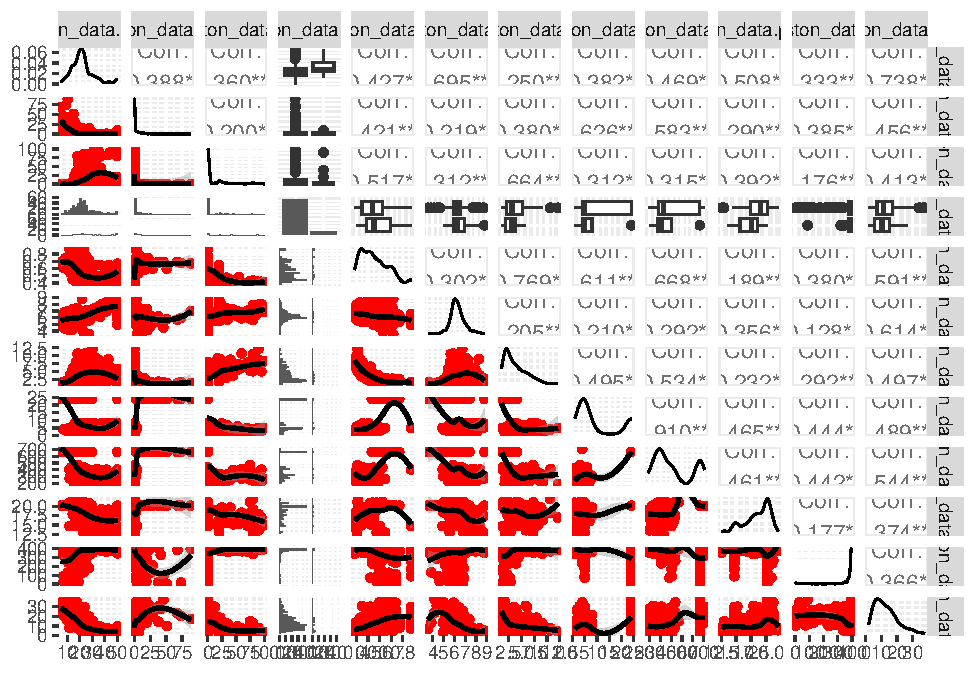
\includegraphics[keepaspectratio]{project_files/figure-latex/unnamed-chunk-17-1.pdf}}

It looks like the variables that might be worth exploring for possible
higher-order relationships with \texttt{medv} are: \texttt{crim},
\texttt{zn}, \texttt{nox}, \texttt{rm}, \texttt{dis}, \texttt{rad},
\texttt{tax}, and \texttt{lstat}. Each of these variables was tested
using second or higher-degree polynomial terms.

\hfill\break

Based on the exploration of potential higher-order relationships for
variables such as \texttt{crim}, \texttt{zn}, \texttt{nox}, \texttt{rm},
\texttt{dis}, \texttt{rad}, \texttt{tax}, and \texttt{lstat}, only the
\textbf{significant polynomial terms} were retained. These significant
higher-order terms were then added to the \textbf{reduced interaction
model} to form an extended model that captures potential
\textbf{non-linear effects} while preserving \textbf{interpretability}.

\begin{longtable}[]{@{}lrrrr@{}}
\caption{Coefficient Estimates from the Higher-Order Interaction
Model}\tabularnewline
\toprule\noalign{}
& Estimate & Std. Error & t value &
Pr(\textgreater\textbar t\textbar) \\
\midrule\noalign{}
\endfirsthead
\toprule\noalign{}
& Estimate & Std. Error & t value &
Pr(\textgreater\textbar t\textbar) \\
\midrule\noalign{}
\endhead
\bottomrule\noalign{}
\endlastfoot
(Intercept) & 9.9501 & 20.6459 & 0.4819 & 0.6301 \\
crim & -7.6931 & 2.6257 & -2.9300 & 0.0036 \\
I(crim\^{}2) & 0.0033 & 0.0010 & 3.4291 & 0.0007 \\
zn & -0.0274 & 0.0449 & -0.6094 & 0.5425 \\
chasYes & 40.8059 & 6.4722 & 6.3049 & 0.0000 \\
nox & -50.9960 & 20.7700 & -2.4553 & 0.0144 \\
I(nox\^{}2) & 37.3520 & 15.9688 & 2.3391 & 0.0197 \\
rm & 5.1164 & 4.4713 & 1.1443 & 0.2531 \\
I(rm\^{}2) & 0.8483 & 0.2501 & 3.3914 & 0.0008 \\
dis & -9.5208 & 1.3265 & -7.1776 & 0.0000 \\
I(dis\^{}2) & 0.1950 & 0.0668 & 2.9183 & 0.0037 \\
rad & 1.4647 & 0.2533 & 5.7819 & 0.0000 \\
tax & -0.0168 & 0.0028 & -6.0234 & 0.0000 \\
ptratio & 4.5064 & 0.7377 & 6.1088 & 0.0000 \\
b & 0.0219 & 0.0061 & 3.5628 & 0.0004 \\
lstat & -5.6167 & 1.1499 & -4.8846 & 0.0000 \\
I(lstat\^{}2) & 0.6351 & 0.1467 & 4.3296 & 0.0000 \\
I(lstat\^{}3) & -0.0354 & 0.0094 & -3.7866 & 0.0002 \\
I(lstat\^{}4) & 0.0009 & 0.0003 & 3.4318 & 0.0007 \\
I(lstat\^{}5) & 0.0000 & 0.0000 & -3.1448 & 0.0018 \\
crim:zn & 0.1002 & 0.1224 & 0.8188 & 0.4133 \\
crim:chasYes & 2.2145 & 0.3103 & 7.1357 & 0.0000 \\
crim:rad & -0.4371 & 0.1336 & -3.2712 & 0.0011 \\
crim:tax & 0.0267 & 0.0086 & 3.1043 & 0.0020 \\
zn:dis & 0.0025 & 0.0066 & 0.3808 & 0.7036 \\
chasYes:nox & -35.3766 & 5.6715 & -6.2377 & 0.0000 \\
chasYes:rm & -3.4379 & 0.7404 & -4.6434 & 0.0000 \\
nox:rad & -1.2613 & 0.3207 & -3.9325 & 0.0001 \\
rm:dis & 0.8557 & 0.1539 & 5.5598 & 0.0000 \\
rm:ptratio & -0.7816 & 0.1137 & -6.8745 & 0.0000 \\
rm:lstat & -0.0730 & 0.0547 & -1.3346 & 0.1826 \\
\url{dis:rad} & -0.0913 & 0.0287 & -3.1778 & 0.0016 \\
\url{dis:lstat} & 0.1575 & 0.0209 & 7.5254 & 0.0000 \\
b:lstat & -0.0008 & 0.0003 & -2.7996 & 0.0053 \\
\end{longtable}

The new insignificant variables were then dropped to get a reduced
higher order interaction model.

\begin{longtable}[]{@{}lrrrr@{}}
\caption{Coefficient Estimates from the Reduced Higher-Order Interaction
Model}\tabularnewline
\toprule\noalign{}
& Estimate & Std. Error & t value &
Pr(\textgreater\textbar t\textbar) \\
\midrule\noalign{}
\endfirsthead
\toprule\noalign{}
& Estimate & Std. Error & t value &
Pr(\textgreater\textbar t\textbar) \\
\midrule\noalign{}
\endhead
\bottomrule\noalign{}
\endlastfoot
(Intercept) & 21.1228 & 18.1497 & 1.1638 & 0.2451 \\
crim & -6.8087 & 2.3071 & -2.9512 & 0.0033 \\
I(crim\^{}2) & 0.0030 & 0.0009 & 3.2112 & 0.0014 \\
chasYes & 40.8986 & 6.4563 & 6.3347 & 0.0000 \\
nox & -45.6887 & 19.3695 & -2.3588 & 0.0187 \\
I(nox\^{}2) & 34.0115 & 15.0189 & 2.2646 & 0.0240 \\
rm & 2.0706 & 3.8551 & 0.5371 & 0.5914 \\
I(rm\^{}2) & 1.0438 & 0.2129 & 4.9031 & 0.0000 \\
dis & -9.6278 & 1.2806 & -7.5182 & 0.0000 \\
I(dis\^{}2) & 0.2099 & 0.0402 & 5.2174 & 0.0000 \\
rad & 1.4358 & 0.2495 & 5.7557 & 0.0000 \\
tax & -0.0167 & 0.0027 & -6.1010 & 0.0000 \\
ptratio & 4.5541 & 0.7094 & 6.4197 & 0.0000 \\
b & 0.0207 & 0.0061 & 3.4008 & 0.0007 \\
lstat & -6.2120 & 0.9861 & -6.2998 & 0.0000 \\
I(lstat\^{}2) & 0.6456 & 0.1438 & 4.4887 & 0.0000 \\
I(lstat\^{}3) & -0.0359 & 0.0092 & -3.8818 & 0.0001 \\
I(lstat\^{}4) & 0.0009 & 0.0003 & 3.4969 & 0.0005 \\
I(lstat\^{}5) & 0.0000 & 0.0000 & -3.1780 & 0.0016 \\
crim:chasYes & 2.2772 & 0.3062 & 7.4366 & 0.0000 \\
crim:rad & -0.3893 & 0.1162 & -3.3501 & 0.0009 \\
crim:tax & 0.0237 & 0.0075 & 3.1680 & 0.0016 \\
chasYes:nox & -35.8644 & 5.6434 & -6.3551 & 0.0000 \\
chasYes:rm & -3.4176 & 0.7377 & -4.6328 & 0.0000 \\
nox:rad & -1.3052 & 0.3164 & -4.1248 & 0.0000 \\
rm:dis & 0.8439 & 0.1468 & 5.7485 & 0.0000 \\
rm:ptratio & -0.7927 & 0.1070 & -7.4074 & 0.0000 \\
\url{dis:rad} & -0.0770 & 0.0271 & -2.8443 & 0.0046 \\
\url{dis:lstat} & 0.1559 & 0.0206 & 7.5497 & 0.0000 \\
b:lstat & -0.0007 & 0.0003 & -2.5465 & 0.0112 \\
\end{longtable}

The higher-order interaction model with significant variables is:

\[
\begin{aligned}
\hat{medv}_i =\ & 36.3411 - 0.1084 \cdot crim_i + 0.0458 \cdot zn_i + 2.7187 \cdot chas_i - 17.3760 \cdot nox_i \\
& + 3.8016 \cdot rm_i - 1.4927 \cdot dis_i + 0.2996 \cdot rad_i - 0.0118 \cdot tax_i - 0.9465 \cdot ptratio_i \\
& + 0.0093 \cdot b_i - 0.5226 \cdot lstat_i
\end{aligned}
\]

where \(chas_{i}\) is 1 if the tract bounds Charles River and 0 if
otherwise

\hfill\break
\hfill\break
\hfill\break
\hfill\break
\hfill\break
\hfill\break

E. \textbf{Testing Multiple Regression Assumptions}\\
The following multiple regression assumptions were tested to check if
the model is trustworthy

\subsection{Linearity Assumption}\label{linearity-assumption}

A scatter plot of the distribution of residuals (errors) vs fitted
values (predicted values) was plotted below

\pandocbounded{\includegraphics[keepaspectratio]{project_files/figure-latex/unnamed-chunk-21-1.pdf}}

There appears to be no pattern of the residuals at all, indicating that
the model passes the linearity assumption that there is a straight-line
(linear) relationship between the predictors and the response.

\subsection{Independence Assumption}\label{independence-assumption}

In the Boston housing dataset, the subjects were not related to time,
space, or group, so we can be pretty sure that their measurements are
independent.

\subsection{Equal Variance Assumption}\label{equal-variance-assumption}

The residuals plot in the linearity assumption section indicates a
smooth fit to the residuals, which is good. In addition to the residuals
plot, a scale-location plot between fitted values and standardized
residuals was also plotted to show if the residuals are spread equally
along the ranges of predictors

\pandocbounded{\includegraphics[keepaspectratio]{project_files/figure-latex/unnamed-chunk-22-1.pdf}}

Based on the plot, we can see that the scale-location plot is quite
horizontal, and there is not any funneling in the residual plot,
indicating equal variance.

The Breusch-Pagan test was then run as a more formal way to assess if we
have homo/heteroscedasticity using the following hypotheses:

\[
\begin{aligned}
H_0:&\mbox{ heteroscedasticity is not present (homoscedasticity)}\\
H_a~:&\mbox{ heteroscedasticity is present} \\
\end{aligned}
\]

\begin{Shaded}
\begin{Highlighting}[]
\FunctionTok{bptest}\NormalTok{(higher\_order\_interaction\_model\_2)}
\end{Highlighting}
\end{Shaded}

\begin{verbatim}
## 
##  studentized Breusch-Pagan test
## 
## data:  higher_order_interaction_model_2
## BP = 70.605, df = 29, p-value = 2.505e-05
\end{verbatim}

The p-value of the Breusch-Pagan test is less than 0.05 (2.505e-05), so
we fail to reject the null hypothesis, indicating we do have
heteroscedasticity.

An attempt to address the heteroscedasticity, in addition to any other
assumption failure will be done after testing all other assumptions.

\subsection{Normality Assumption}\label{normality-assumption}

The multiple linear regression analysis requires that the errors between
observed and predicted values (i.e., the residuals of the regression)
should be normally distributed.

A histogram and q-q plot were developed to check if the residuals were
normally distributed or not.

\pandocbounded{\includegraphics[keepaspectratio]{project_files/figure-latex/unnamed-chunk-24-1.pdf}}

\pandocbounded{\includegraphics[keepaspectratio]{project_files/figure-latex/unnamed-chunk-25-1.pdf}}

Based on the plots above, it appears the residuals are not normal. A
\textbf{Shapiro-Wilk test} was conducted to assess whether the residuals
from the model are normally distributed.

\subsubsection{Hypotheses}\label{hypotheses}

\[
\begin{aligned}
H_0\!: & \text{ The residuals are normally distributed} \\
H_a\!: & \text{ The residuals are not normally distributed}
\end{aligned}
\]

\begin{verbatim}
## 
##  Shapiro-Wilk normality test
## 
## data:  residuals(higher_order_interaction_model_2)
## W = 0.94232, p-value = 4.088e-13
\end{verbatim}

The p-value of the Shapiro-Wilk normality test is less than 0.05
(4.088e-13), so we fail to reject the null hypothesis, indicating we do
not have normality.

An attempt to address the normality will be done after testing all other
assumptions.

\hfill\break
\hfill\break
\hfill\break

\subsection{Outliers}\label{outliers}

The below approaches were explored to find and evaluate outliers or
influential points.

\begin{enumerate}
\def\labelenumi{\arabic{enumi}.}
\tightlist
\item
  Residuals vs Leverage Plot
\end{enumerate}

\pandocbounded{\includegraphics[keepaspectratio]{project_files/figure-latex/unnamed-chunk-27-1.pdf}}

The plot above shows that all cases are well inside of the Cook's
distance lines, indicating no outliers or no influential points.

\begin{enumerate}
\def\labelenumi{\arabic{enumi}.}
\setcounter{enumi}{1}
\tightlist
\item
  Cook's Distance
\end{enumerate}

\pandocbounded{\includegraphics[keepaspectratio]{project_files/figure-latex/unnamed-chunk-28-1.pdf}}

Based on the consensus that a value of more than 1 indicates an
influential value, the cook's distance plot above indicates there are no
influential values.

\begin{enumerate}
\def\labelenumi{\arabic{enumi}.}
\setcounter{enumi}{2}
\tightlist
\item
  Leverage points
\end{enumerate}

\begin{verbatim}
## [1] "h_I>2p/n, outliers are"
\end{verbatim}

\begin{verbatim}
##         9        49       103       142       143       144       145       148 
## 0.2354513 0.2211416 0.1189061 0.2196870 0.2272326 0.1541038 0.1270919 0.1264748 
##       153       155       156       160       162       163       164       166 
## 0.3272566 0.2732434 0.2282326 0.1407945 0.1557776 0.1974755 0.2298756 0.1369647 
##       210       212       226       254       258       263       266       274 
## 0.1509071 0.1421784 0.1340614 0.2676467 0.1906601 0.1340792 0.1309452 0.1223700 
##       283       284       311       353       354       355       356       357 
## 0.1225426 0.1912266 0.2467671 0.1213298 0.2761866 0.1525040 0.1316790 0.3444005 
##       359       365       366       368       369       370       371       373 
## 0.1311273 0.4626355 0.2995252 0.1896458 0.1789528 0.1684122 0.2365689 0.3381414 
##       374       375       381       399       406       407       411       413 
## 0.1742488 0.6361285 0.6384477 0.1198824 0.1776729 0.1275039 0.2407394 0.2526555 
##       415       419       428       439       491 
## 0.4148876 0.2481005 0.1393357 0.1917905 0.1364389
\end{verbatim}

\begin{verbatim}
## [1] "h_I>3p/n, outliers are"
\end{verbatim}

\begin{verbatim}
##         9        49       142       143       153       155       156       163 
## 0.2354513 0.2211416 0.2196870 0.2272326 0.3272566 0.2732434 0.2282326 0.1974755 
##       164       254       258       284       311       354       357       365 
## 0.2298756 0.2676467 0.1906601 0.1912266 0.2467671 0.2761866 0.3444005 0.4626355 
##       366       368       369       371       373       375       381       411 
## 0.2995252 0.1896458 0.1789528 0.2365689 0.3381414 0.6361285 0.6384477 0.2407394 
##       413       415       419       439 
## 0.2526555 0.4148876 0.2481005 0.1917905
\end{verbatim}

\pandocbounded{\includegraphics[keepaspectratio]{project_files/figure-latex/unnamed-chunk-31-1.pdf}}

Based on the above plot, it appears we have high leverage points but
none of them appear to be particularly influential (no points with a
concerning cooks distance). Hence, it appears we do not have any
outliers that could pose problems.

\subsection{Dealing with Heteroscedasticity and
Normality}\label{dealing-with-heteroscedasticity-and-normality}

Now that all multiple regression assumptions have been tested to check
if the model is trustworthy, we then made attempts to address the
heteroscedasticity and lack of normality.

We started by making a log transformation of the predictor so the
difference between big and small numbers relatively becomes small.

\begin{longtable}[]{@{}lrrrr@{}}
\caption{Coefficient Estimates from the Log-Transformed Higher-Order
Interaction Model}\tabularnewline
\toprule\noalign{}
& Estimate & Std. Error & t value &
Pr(\textgreater\textbar t\textbar) \\
\midrule\noalign{}
\endfirsthead
\toprule\noalign{}
& Estimate & Std. Error & t value &
Pr(\textgreater\textbar t\textbar) \\
\midrule\noalign{}
\endhead
\bottomrule\noalign{}
\endlastfoot
(Intercept) & 4.4823 & 0.8708 & 5.1471 & 0.0000 \\
crim & -0.2790 & 0.1107 & -2.5207 & 0.0120 \\
I(crim\^{}2) & 0.0002 & 0.0000 & 4.4711 & 0.0000 \\
chasYes & 1.5587 & 0.3098 & 5.0315 & 0.0000 \\
nox & -1.8645 & 0.9294 & -2.0063 & 0.0454 \\
I(nox\^{}2) & 1.3414 & 0.7206 & 1.8614 & 0.0633 \\
rm & -0.1186 & 0.1850 & -0.6412 & 0.5217 \\
I(rm\^{}2) & 0.0342 & 0.0102 & 3.3530 & 0.0009 \\
dis & -0.4052 & 0.0614 & -6.5949 & 0.0000 \\
I(dis\^{}2) & 0.0081 & 0.0019 & 4.2099 & 0.0000 \\
rad & 0.0666 & 0.0120 & 5.5602 & 0.0000 \\
tax & -0.0008 & 0.0001 & -5.9526 & 0.0000 \\
ptratio & 0.0917 & 0.0340 & 2.6942 & 0.0073 \\
b & 0.0007 & 0.0003 & 2.5487 & 0.0111 \\
lstat & -0.1671 & 0.0473 & -3.5310 & 0.0005 \\
I(lstat\^{}2) & 0.0160 & 0.0069 & 2.3226 & 0.0206 \\
I(lstat\^{}3) & -0.0009 & 0.0004 & -1.9904 & 0.0471 \\
I(lstat\^{}4) & 0.0000 & 0.0000 & 1.6681 & 0.0960 \\
I(lstat\^{}5) & 0.0000 & 0.0000 & -1.3179 & 0.1882 \\
crim:chasYes & 0.0801 & 0.0147 & 5.4500 & 0.0000 \\
crim:rad & -0.0158 & 0.0056 & -2.8256 & 0.0049 \\
crim:tax & 0.0009 & 0.0004 & 2.6413 & 0.0085 \\
chasYes:nox & -1.3425 & 0.2708 & -4.9581 & 0.0000 \\
chasYes:rm & -0.1302 & 0.0354 & -3.6790 & 0.0003 \\
nox:rad & -0.0613 & 0.0152 & -4.0392 & 0.0001 \\
rm:dis & 0.0375 & 0.0070 & 5.3256 & 0.0000 \\
rm:ptratio & -0.0179 & 0.0051 & -3.4928 & 0.0005 \\
\url{dis:rad} & -0.0026 & 0.0013 & -2.0157 & 0.0444 \\
\url{dis:lstat} & 0.0060 & 0.0010 & 6.0399 & 0.0000 \\
b:lstat & 0.0000 & 0.0000 & -1.5860 & 0.1134 \\
\end{longtable}

Some insignificant variables were observed after the log transformation,
which were subsequently dropped from the model

\begin{longtable}[]{@{}lrrrr@{}}
\caption{Coefficient Estimates from the Final Reduced Log-Transformed
Model}\tabularnewline
\toprule\noalign{}
& Estimate & Std. Error & t value &
Pr(\textgreater\textbar t\textbar) \\
\midrule\noalign{}
\endfirsthead
\toprule\noalign{}
& Estimate & Std. Error & t value &
Pr(\textgreater\textbar t\textbar) \\
\midrule\noalign{}
\endhead
\bottomrule\noalign{}
\endlastfoot
(Intercept) & 4.7592 & 0.8451 & 5.6317 & 0.0000 \\
crim & -0.3149 & 0.1078 & -2.9224 & 0.0036 \\
I(crim\^{}2) & 0.0002 & 0.0000 & 4.1092 & 0.0000 \\
chasYes & 1.5244 & 0.3111 & 4.8996 & 0.0000 \\
nox & -0.3748 & 0.2194 & -1.7085 & 0.0882 \\
rm & -0.2175 & 0.1789 & -1.2154 & 0.2248 \\
I(rm\^{}2) & 0.0374 & 0.0101 & 3.6981 & 0.0002 \\
dis & -0.4104 & 0.0585 & -7.0146 & 0.0000 \\
I(dis\^{}2) & 0.0085 & 0.0018 & 4.7124 & 0.0000 \\
rad & 0.0459 & 0.0081 & 5.6678 & 0.0000 \\
tax & -0.0008 & 0.0001 & -5.9706 & 0.0000 \\
ptratio & 0.0682 & 0.0325 & 2.0953 & 0.0367 \\
b & 0.0003 & 0.0001 & 3.3344 & 0.0009 \\
lstat & -0.1217 & 0.0243 & -4.9996 & 0.0000 \\
I(lstat\^{}2) & 0.0074 & 0.0024 & 3.1177 & 0.0019 \\
I(lstat\^{}3) & -0.0003 & 0.0001 & -3.2375 & 0.0013 \\
I(lstat\^{}4) & 0.0000 & 0.0000 & 3.5399 & 0.0004 \\
crim:chasYes & 0.0835 & 0.0147 & 5.6817 & 0.0000 \\
crim:rad & -0.0174 & 0.0053 & -3.2674 & 0.0012 \\
crim:tax & 0.0011 & 0.0003 & 3.0806 & 0.0022 \\
chasYes:nox & -1.3024 & 0.2711 & -4.8047 & 0.0000 \\
chasYes:rm & -0.1282 & 0.0354 & -3.6239 & 0.0003 \\
nox:rad & -0.0408 & 0.0129 & -3.1648 & 0.0017 \\
rm:dis & 0.0370 & 0.0070 & 5.2671 & 0.0000 \\
rm:ptratio & -0.0149 & 0.0050 & -2.9978 & 0.0029 \\
\url{dis:lstat} & 0.0056 & 0.0009 & 5.9387 & 0.0000 \\
\end{longtable}

The log-transformed model was tested for homoscedasticity and normality.

\begin{longtable}[]{@{}lrrrr@{}}
\caption{Coefficient Estimates from the Reduced Log-Transformed
Higher-Order Interaction Model}\tabularnewline
\toprule\noalign{}
& Estimate & Std. Error & t value &
Pr(\textgreater\textbar t\textbar) \\
\midrule\noalign{}
\endfirsthead
\toprule\noalign{}
& Estimate & Std. Error & t value &
Pr(\textgreater\textbar t\textbar) \\
\midrule\noalign{}
\endhead
\bottomrule\noalign{}
\endlastfoot
(Intercept) & 4.7592 & 0.8451 & 5.6317 & 0.0000 \\
crim & -0.3149 & 0.1078 & -2.9224 & 0.0036 \\
I(crim\^{}2) & 0.0002 & 0.0000 & 4.1092 & 0.0000 \\
chasYes & 1.5244 & 0.3111 & 4.8996 & 0.0000 \\
nox & -0.3748 & 0.2194 & -1.7085 & 0.0882 \\
rm & -0.2175 & 0.1789 & -1.2154 & 0.2248 \\
I(rm\^{}2) & 0.0374 & 0.0101 & 3.6981 & 0.0002 \\
dis & -0.4104 & 0.0585 & -7.0146 & 0.0000 \\
I(dis\^{}2) & 0.0085 & 0.0018 & 4.7124 & 0.0000 \\
rad & 0.0459 & 0.0081 & 5.6678 & 0.0000 \\
tax & -0.0008 & 0.0001 & -5.9706 & 0.0000 \\
ptratio & 0.0682 & 0.0325 & 2.0953 & 0.0367 \\
b & 0.0003 & 0.0001 & 3.3344 & 0.0009 \\
lstat & -0.1217 & 0.0243 & -4.9996 & 0.0000 \\
I(lstat\^{}2) & 0.0074 & 0.0024 & 3.1177 & 0.0019 \\
I(lstat\^{}3) & -0.0003 & 0.0001 & -3.2375 & 0.0013 \\
I(lstat\^{}4) & 0.0000 & 0.0000 & 3.5399 & 0.0004 \\
crim:chasYes & 0.0835 & 0.0147 & 5.6817 & 0.0000 \\
crim:rad & -0.0174 & 0.0053 & -3.2674 & 0.0012 \\
crim:tax & 0.0011 & 0.0003 & 3.0806 & 0.0022 \\
chasYes:nox & -1.3024 & 0.2711 & -4.8047 & 0.0000 \\
chasYes:rm & -0.1282 & 0.0354 & -3.6239 & 0.0003 \\
nox:rad & -0.0408 & 0.0129 & -3.1648 & 0.0017 \\
rm:dis & 0.0370 & 0.0070 & 5.2671 & 0.0000 \\
rm:ptratio & -0.0149 & 0.0050 & -2.9978 & 0.0029 \\
\url{dis:lstat} & 0.0056 & 0.0009 & 5.9387 & 0.0000 \\
\end{longtable}

The p-value of the Breusch-Pagan test is less than 0.05 (4.085e-07),
indicating we still have heteroscedasticity.

\begin{verbatim}
## 
##  Shapiro-Wilk normality test
## 
## data:  residuals(higher_order_interaction_model_log_2)
## W = 0.95209, p-value = 9.614e-12
\end{verbatim}

The p-value of the Shapiro-Wilk normality test is less than 0.05
(9.614e-12), so we fail to reject the null hypothesis, indicating we do
not have normality.

Since the log-transformation approach did not resolve the
heteroscedasticity or lack of normality, we then explored the Box-Cox
transformations approach by identifying \(\hat{\lambda}\), the maximum
likelihood estimate of \(\lambda\) to use in the power transformation

\pandocbounded{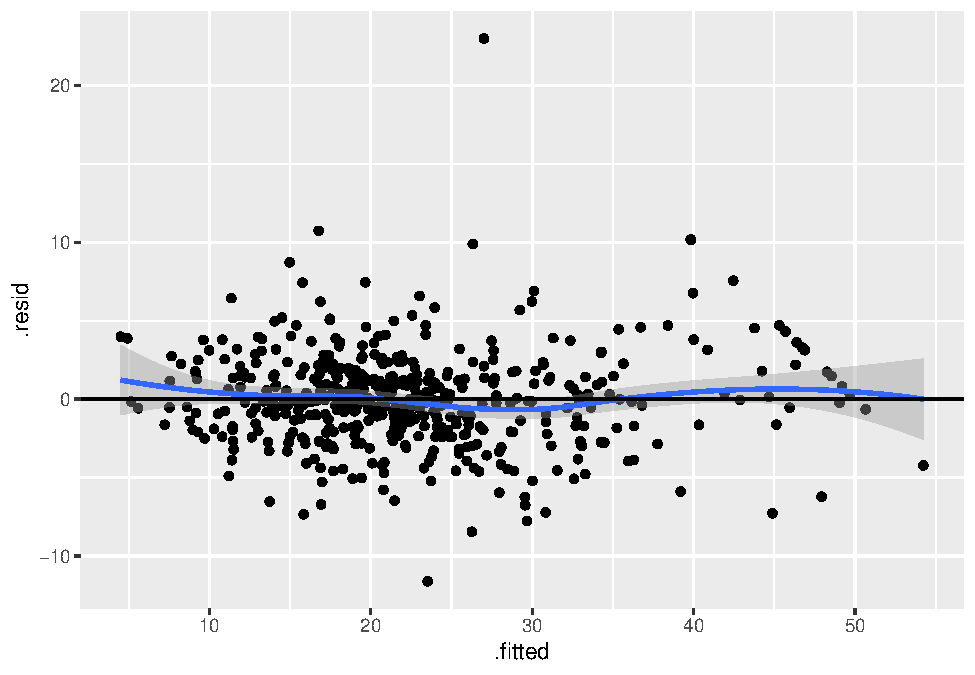
\includegraphics[keepaspectratio]{project_files/figure-latex/unnamed-chunk-36-1.pdf}}

\begin{verbatim}
## [1] 0.4949495
\end{verbatim}

The best lambda estimate was then used to transform the model as
follows:

\begin{longtable}[]{@{}lrrrr@{}}
\caption{Coefficient Estimates from the Box-Cox Transformed Higher-Order
Interaction Model}\tabularnewline
\toprule\noalign{}
& Estimate & Std. Error & t value &
Pr(\textgreater\textbar t\textbar) \\
\midrule\noalign{}
\endfirsthead
\toprule\noalign{}
& Estimate & Std. Error & t value &
Pr(\textgreater\textbar t\textbar) \\
\midrule\noalign{}
\endhead
\bottomrule\noalign{}
\endlastfoot
(Intercept) & 10.4380 & 3.6864 & 2.8315 & 0.0048 \\
crim & -1.3006 & 0.4686 & -2.7754 & 0.0057 \\
I(crim\^{}2) & 0.0007 & 0.0002 & 3.8987 & 0.0001 \\
chasYes & 7.6844 & 1.3113 & 5.8600 & 0.0000 \\
nox & -8.8470 & 3.9341 & -2.2488 & 0.0250 \\
I(nox\^{}2) & 6.3975 & 3.0505 & 2.0972 & 0.0365 \\
rm & -0.0319 & 0.7830 & -0.0407 & 0.9675 \\
I(rm\^{}2) & 0.1788 & 0.0432 & 4.1351 & 0.0000 \\
dis & -1.9261 & 0.2601 & -7.4052 & 0.0000 \\
I(dis\^{}2) & 0.0400 & 0.0082 & 4.8998 & 0.0000 \\
rad & 0.2896 & 0.0507 & 5.7164 & 0.0000 \\
tax & -0.0035 & 0.0006 & -6.2155 & 0.0000 \\
ptratio & 0.6587 & 0.1441 & 4.5718 & 0.0000 \\
b & 0.0039 & 0.0012 & 3.1498 & 0.0017 \\
lstat & -0.9961 & 0.2003 & -4.9734 & 0.0000 \\
I(lstat\^{}2) & 0.1004 & 0.0292 & 3.4383 & 0.0006 \\
I(lstat\^{}3) & -0.0056 & 0.0019 & -2.9802 & 0.0030 \\
I(lstat\^{}4) & 0.0001 & 0.0001 & 2.6395 & 0.0086 \\
I(lstat\^{}5) & 0.0000 & 0.0000 & -2.3135 & 0.0211 \\
crim:chasYes & 0.4094 & 0.0622 & 6.5834 & 0.0000 \\
crim:rad & -0.0734 & 0.0236 & -3.1094 & 0.0020 \\
crim:tax & 0.0045 & 0.0015 & 2.9339 & 0.0035 \\
chasYes:nox & -6.6660 & 1.1462 & -5.8156 & 0.0000 \\
chasYes:rm & -0.6423 & 0.1498 & -4.2870 & 0.0000 \\
nox:rad & -0.2647 & 0.0643 & -4.1180 & 0.0000 \\
rm:dis & 0.1742 & 0.0298 & 5.8435 & 0.0000 \\
rm:ptratio & -0.1198 & 0.0217 & -5.5096 & 0.0000 \\
\url{dis:rad} & -0.0131 & 0.0055 & -2.3742 & 0.0180 \\
\url{dis:lstat} & 0.0292 & 0.0042 & 6.9726 & 0.0000 \\
b:lstat & -0.0001 & 0.0001 & -2.1840 & 0.0295 \\
\end{longtable}

The best lambda transformed model was then tested for homoscedasticity
and normality.

\begin{verbatim}
## 
##  studentized Breusch-Pagan test
## 
## data:  higher_order_interaction_model_2_box
## BP = 68.228, df = 29, p-value = 5.277e-05
\end{verbatim}

The p-value of the Breusch-Pagan test is less than 0.05 (5.277e-05),
indicating we still have heteroscedasticity.

\begin{verbatim}
## 
##  Shapiro-Wilk normality test
## 
## data:  residuals(higher_order_interaction_model_2_box)
## W = 0.96285, p-value = 5.297e-10
\end{verbatim}

The p-value of the Shapiro-Wilk normality test is less than 0.05
(5.297e-10), so we fail to reject the null hypothesis, indicating we do
not have normality.

Since the box-cox transformation approach did not resolve the
heteroscedasticity or lack of normality also, we then explored the
weighted least squares regression method, which is an application of the
more general concept of generalized least squares. This method gives
less weight to observations with high variance as follows:

\begin{longtable}[]{@{}lrrrr@{}}
\caption{Coefficient Estimates from the Weighted Least Squares (WLS)
Model}\tabularnewline
\toprule\noalign{}
& Estimate & Std. Error & t value &
Pr(\textgreater\textbar t\textbar) \\
\midrule\noalign{}
\endfirsthead
\toprule\noalign{}
& Estimate & Std. Error & t value &
Pr(\textgreater\textbar t\textbar) \\
\midrule\noalign{}
\endhead
\bottomrule\noalign{}
\endlastfoot
(Intercept) & 62.6407 & 18.5326 & 3.3800 & 0.0008 \\
crim & -5.8644 & 1.8633 & -3.1473 & 0.0018 \\
I(crim\^{}2) & 0.0033 & 0.0011 & 3.0125 & 0.0027 \\
chasYes & 25.9603 & 7.1304 & 3.6408 & 0.0003 \\
nox & -32.3226 & 14.7937 & -2.1849 & 0.0294 \\
I(nox\^{}2) & 19.5057 & 12.3357 & 1.5812 & 0.1145 \\
rm & -10.0911 & 4.2774 & -2.3592 & 0.0187 \\
I(rm\^{}2) & 1.7307 & 0.2554 & 6.7774 & 0.0000 \\
dis & -7.4567 & 1.1012 & -6.7717 & 0.0000 \\
I(dis\^{}2) & 0.1581 & 0.0337 & 4.6951 & 0.0000 \\
rad & 0.8730 & 0.2617 & 3.3355 & 0.0009 \\
tax & -0.0130 & 0.0021 & -6.1216 & 0.0000 \\
ptratio & 3.1064 & 0.6968 & 4.4583 & 0.0000 \\
b & 0.0199 & 0.0056 & 3.5426 & 0.0004 \\
lstat & -5.0624 & 0.8233 & -6.1488 & 0.0000 \\
I(lstat\^{}2) & 0.5210 & 0.1195 & 4.3607 & 0.0000 \\
I(lstat\^{}3) & -0.0281 & 0.0077 & -3.6491 & 0.0003 \\
I(lstat\^{}4) & 0.0007 & 0.0002 & 3.1929 & 0.0015 \\
I(lstat\^{}5) & 0.0000 & 0.0000 & -2.8414 & 0.0047 \\
crim:chasYes & 1.6158 & 0.3828 & 4.2208 & 0.0000 \\
crim:rad & -0.3063 & 0.1045 & -2.9308 & 0.0035 \\
crim:tax & 0.0193 & 0.0064 & 3.0024 & 0.0028 \\
chasYes:nox & -25.0754 & 5.9957 & -4.1823 & 0.0000 \\
chasYes:rm & -1.9067 & 0.8498 & -2.2437 & 0.0253 \\
nox:rad & -0.6934 & 0.3302 & -2.1002 & 0.0362 \\
rm:dis & 0.6555 & 0.1270 & 5.1618 & 0.0000 \\
rm:ptratio & -0.5768 & 0.1088 & -5.3033 & 0.0000 \\
\url{dis:rad} & -0.0335 & 0.0245 & -1.3692 & 0.1716 \\
\url{dis:lstat} & 0.1010 & 0.0165 & 6.1227 & 0.0000 \\
b:lstat & -0.0007 & 0.0003 & -2.5663 & 0.0106 \\
\end{longtable}

Some insignificant variables were observed, which were subsequently
dropped from the model

\begin{longtable}[]{@{}lrrrr@{}}
\caption{Coefficient Estimates from the Final Weighted Least Squares
(WLS) Model}\tabularnewline
\toprule\noalign{}
& Estimate & Std. Error & t value &
Pr(\textgreater\textbar t\textbar) \\
\midrule\noalign{}
\endfirsthead
\toprule\noalign{}
& Estimate & Std. Error & t value &
Pr(\textgreater\textbar t\textbar) \\
\midrule\noalign{}
\endhead
\bottomrule\noalign{}
\endlastfoot
(Intercept) & 68.5135 & 18.2808 & 3.7478 & 0.0002 \\
crim & -6.2359 & 1.8136 & -3.4385 & 0.0006 \\
I(crim\^{}2) & 0.0028 & 0.0010 & 2.7280 & 0.0066 \\
chasYes & 24.9904 & 7.1315 & 3.5042 & 0.0005 \\
nox & -12.3056 & 3.9348 & -3.1274 & 0.0019 \\
rm & -12.0553 & 4.1541 & -2.9020 & 0.0039 \\
I(rm\^{}2) & 1.8107 & 0.2524 & 7.1752 & 0.0000 \\
dis & -7.5744 & 1.0829 & -6.9944 & 0.0000 \\
I(dis\^{}2) & 0.1672 & 0.0329 & 5.0777 & 0.0000 \\
rad & 0.5139 & 0.1532 & 3.3537 & 0.0009 \\
tax & -0.0128 & 0.0021 & -6.1063 & 0.0000 \\
ptratio & 2.7413 & 0.6697 & 4.0932 & 0.0000 \\
b & 0.0194 & 0.0056 & 3.4682 & 0.0006 \\
lstat & -4.9962 & 0.8246 & -6.0589 & 0.0000 \\
I(lstat\^{}2) & 0.5105 & 0.1196 & 4.2674 & 0.0000 \\
I(lstat\^{}3) & -0.0274 & 0.0077 & -3.5548 & 0.0004 \\
I(lstat\^{}4) & 0.0007 & 0.0002 & 3.1045 & 0.0020 \\
I(lstat\^{}5) & 0.0000 & 0.0000 & -2.7640 & 0.0059 \\
crim:chasYes & 1.5647 & 0.3825 & 4.0912 & 0.0001 \\
crim:rad & -0.3414 & 0.0995 & -3.4308 & 0.0007 \\
crim:tax & 0.0211 & 0.0062 & 3.4308 & 0.0007 \\
chasYes:nox & -23.3711 & 5.9264 & -3.9436 & 0.0001 \\
chasYes:rm & -1.8831 & 0.8507 & -2.2135 & 0.0273 \\
nox:rad & -0.2886 & 0.2507 & -1.1515 & 0.2501 \\
rm:dis & 0.6478 & 0.1272 & 5.0910 & 0.0000 \\
rm:ptratio & -0.5280 & 0.1056 & -4.9986 & 0.0000 \\
\url{dis:lstat} & 0.0968 & 0.0164 & 5.9095 & 0.0000 \\
b:lstat & -0.0007 & 0.0003 & -2.5246 & 0.0119 \\
\end{longtable}

A further insignificant variables was observed, which was also dropped
from the model

\begin{longtable}[]{@{}lrrrr@{}}
\caption{Coefficient Estimates from the Final Reduced WLS
Model}\tabularnewline
\toprule\noalign{}
& Estimate & Std. Error & t value &
Pr(\textgreater\textbar t\textbar) \\
\midrule\noalign{}
\endfirsthead
\toprule\noalign{}
& Estimate & Std. Error & t value &
Pr(\textgreater\textbar t\textbar) \\
\midrule\noalign{}
\endhead
\bottomrule\noalign{}
\endlastfoot
(Intercept) & 72.0267 & 18.0305 & 3.9947 & 0.0001 \\
crim & -6.2812 & 1.8137 & -3.4631 & 0.0006 \\
I(crim\^{}2) & 0.0030 & 0.0010 & 2.9893 & 0.0029 \\
chasYes & 24.6121 & 7.1263 & 3.4537 & 0.0006 \\
nox & -15.3681 & 2.9009 & -5.2978 & 0.0000 \\
rm & -12.4565 & 4.1409 & -3.0082 & 0.0028 \\
I(rm\^{}2) & 1.8274 & 0.2520 & 7.2507 & 0.0000 \\
dis & -7.7389 & 1.0738 & -7.2068 & 0.0000 \\
I(dis\^{}2) & 0.1715 & 0.0327 & 5.2422 & 0.0000 \\
rad & 0.3466 & 0.0488 & 7.1037 & 0.0000 \\
tax & -0.0130 & 0.0021 & -6.2272 & 0.0000 \\
ptratio & 2.7039 & 0.6692 & 4.0408 & 0.0001 \\
b & 0.0199 & 0.0056 & 3.5703 & 0.0004 \\
lstat & -4.9514 & 0.8240 & -6.0091 & 0.0000 \\
I(lstat\^{}2) & 0.5050 & 0.1196 & 4.2230 & 0.0000 \\
I(lstat\^{}3) & -0.0271 & 0.0077 & -3.5133 & 0.0005 \\
I(lstat\^{}4) & 0.0007 & 0.0002 & 3.0642 & 0.0023 \\
I(lstat\^{}5) & 0.0000 & 0.0000 & -2.7247 & 0.0067 \\
crim:chasYes & 1.4847 & 0.3762 & 3.9463 & 0.0001 \\
crim:rad & -0.3624 & 0.0979 & -3.7035 & 0.0002 \\
crim:tax & 0.0219 & 0.0061 & 3.5816 & 0.0004 \\
chasYes:nox & -22.7484 & 5.9036 & -3.8533 & 0.0001 \\
chasYes:rm & -1.8725 & 0.8510 & -2.2004 & 0.0283 \\
rm:dis & 0.6587 & 0.1269 & 5.1899 & 0.0000 \\
rm:ptratio & -0.5220 & 0.1055 & -4.9456 & 0.0000 \\
\url{dis:lstat} & 0.0983 & 0.0163 & 6.0181 & 0.0000 \\
b:lstat & -0.0007 & 0.0003 & -2.6107 & 0.0093 \\
\end{longtable}

The model derived from the weighted least squares regression method was
tested for homoscedasticity and normality.

\begin{verbatim}
## 
##  studentized Breusch-Pagan test
## 
## data:  higher_order_interaction_model_wls_3
## BP = 11.552, df = 26, p-value = 0.9934
\end{verbatim}

The p-value of the Breusch-Pagan test is greater than 0.05 (0.9934),
indicating we now finally have homoscedasticity.

\begin{verbatim}
## 
##  Shapiro-Wilk normality test
## 
## data:  residuals(higher_order_interaction_model_wls_3)
## W = 0.88798, p-value < 2.2e-16
\end{verbatim}

The p-value of the Shapiro-Wilk normality test is less than 0.05
(9.614e-12), indicating we still do not have normality.

Even though we do not have normality, due to our dataset having a large
sample size, the Central Limit Theorem can compensate for the
non-normality in the residuals. The Central Limit Theorem states that,
for a sufficiently large sample from a population, the sampling
distribution of the estimates tends to be normal, regardless of the
underlying population distribution. This suggests that the residuals do
not need to be perfectly normal.

The linearity and outliers assumptions would be tested again to confirm
they are still met

\section{Linearity Assumption}\label{linearity-assumption-1}

\pandocbounded{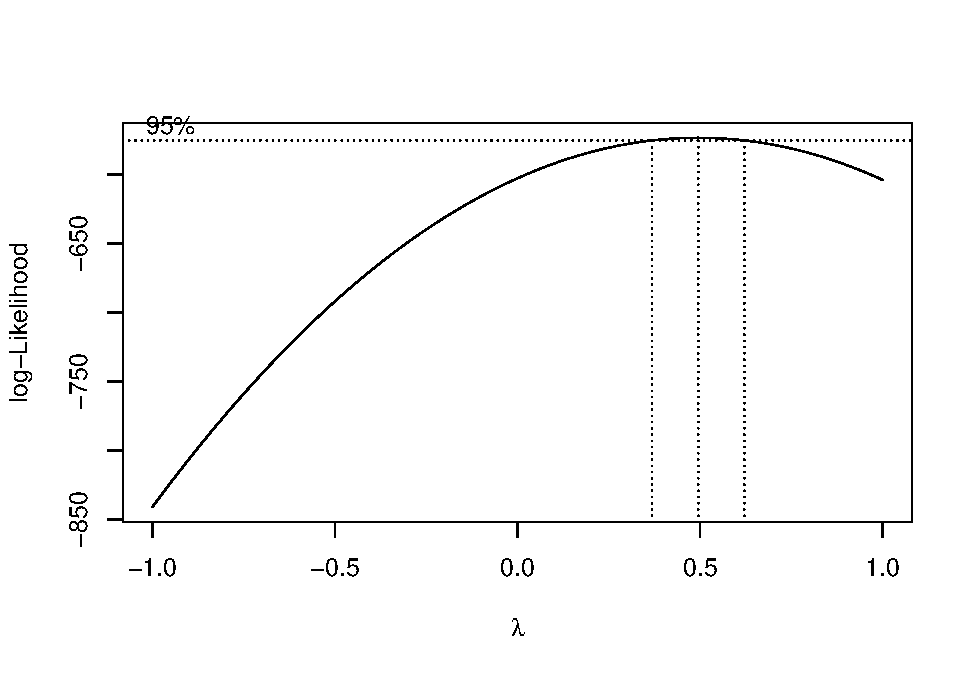
\includegraphics[keepaspectratio]{project_files/figure-latex/unnamed-chunk-49-1.pdf}}

Based on the updated model, there appears to be no pattern of the
residuals at all, indicating that the model still passes the linearity
assumption that there is a straight-line (linear) relationship between
the predictors and the response.

\pandocbounded{\includegraphics[keepaspectratio]{project_files/figure-latex/unnamed-chunk-50-1.pdf}}

\subsection{Outliers}\label{outliers-1}

\begin{enumerate}
\def\labelenumi{\arabic{enumi}.}
\tightlist
\item
  Residuals vs Leverage Plot
\end{enumerate}

\pandocbounded{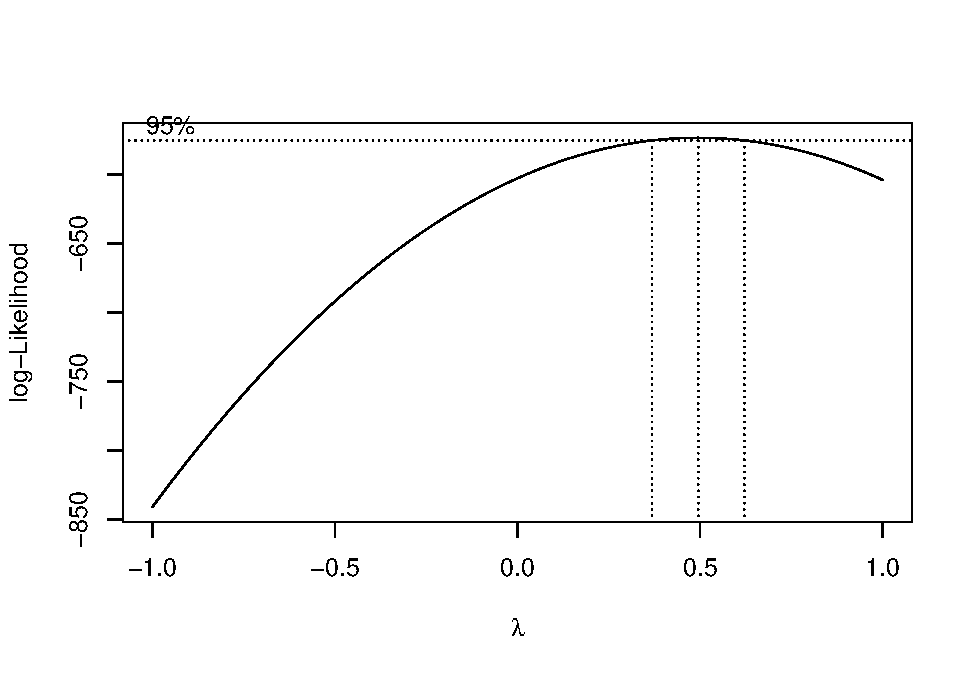
\includegraphics[keepaspectratio]{project_files/figure-latex/unnamed-chunk-51-1.pdf}}

The plot above shows that all cases are well inside of the Cook's
distance lines, indicating no outliers or no influential points.

\begin{enumerate}
\def\labelenumi{\arabic{enumi}.}
\setcounter{enumi}{1}
\tightlist
\item
  Cook's Distance
\end{enumerate}

\pandocbounded{\includegraphics[keepaspectratio]{project_files/figure-latex/unnamed-chunk-52-1.pdf}}

Based on the consensus that a value of more than 1 indicates an
influential value, the cook's distance plot above indicates there are
still no influential values.

\begin{enumerate}
\def\labelenumi{\arabic{enumi}.}
\setcounter{enumi}{2}
\tightlist
\item
  Leverage points
\end{enumerate}

\begin{verbatim}
## [1] "h_I>2p/n, outliers are"
\end{verbatim}

\begin{verbatim}
##         9        49       103       142       143       144       145       148 
## 0.2354513 0.2211416 0.1189061 0.2196870 0.2272326 0.1541038 0.1270919 0.1264748 
##       153       155       156       160       162       163       164       166 
## 0.3272566 0.2732434 0.2282326 0.1407945 0.1557776 0.1974755 0.2298756 0.1369647 
##       210       212       226       254       258       263       266       274 
## 0.1509071 0.1421784 0.1340614 0.2676467 0.1906601 0.1340792 0.1309452 0.1223700 
##       283       284       311       353       354       355       356       357 
## 0.1225426 0.1912266 0.2467671 0.1213298 0.2761866 0.1525040 0.1316790 0.3444005 
##       359       365       366       368       369       370       371       373 
## 0.1311273 0.4626355 0.2995252 0.1896458 0.1789528 0.1684122 0.2365689 0.3381414 
##       374       375       381       399       406       407       411       413 
## 0.1742488 0.6361285 0.6384477 0.1198824 0.1776729 0.1275039 0.2407394 0.2526555 
##       415       419       428       439       491 
## 0.4148876 0.2481005 0.1393357 0.1917905 0.1364389
\end{verbatim}

\begin{verbatim}
## [1] "h_I>3p/n, outliers are"
\end{verbatim}

\begin{verbatim}
##         9        49       142       143       153       155       156       163 
## 0.2354513 0.2211416 0.2196870 0.2272326 0.3272566 0.2732434 0.2282326 0.1974755 
##       164       254       258       284       311       354       357       365 
## 0.2298756 0.2676467 0.1906601 0.1912266 0.2467671 0.2761866 0.3444005 0.4626355 
##       366       368       369       371       373       375       381       411 
## 0.2995252 0.1896458 0.1789528 0.2365689 0.3381414 0.6361285 0.6384477 0.2407394 
##       413       415       419       439 
## 0.2526555 0.4148876 0.2481005 0.1917905
\end{verbatim}

\pandocbounded{\includegraphics[keepaspectratio]{project_files/figure-latex/unnamed-chunk-55-1.pdf}}

Based on the above plot, it appears we still have high leverage points
but none of them appear to be particularly influential (no points with a
concerning cooks distance). Hence, it appears we do not have any
outliers that could pose problems.

\section{4. CONCLUSION AND DISCUSSION}\label{conclusion-and-discussion}

We developed a predictive model using \textbf{multiple linear
regression} to estimate the median value of owner-occupied homes in
Boston based on 13 housing and neighborhood features. After loading the
data, we tested for \textbf{multicollinearity}, and none was detected.

We then built a \textbf{baseline additive model} and refined it by
removing insignificant predictors. Interaction effects were explored,
and a \textbf{reduced interaction model} was selected based on predictor
significance and model performance. Next, we examined
\textbf{higher-order terms} to capture non-linear relationships,
iteratively refining the model to retain only statistically significant
predictors.

Finally, we tested the \textbf{multiple regression
assumptions}---linearity, independence, equal variance, normality, and
presence of outliers. While the final model satisfied most assumptions,
the \textbf{residuals remained non-normal} despite attempts to correct
this using log transformation, Box-Cox transformation, and
\textbf{weighted least squares (WLS)} regression.

Ultimately, the \textbf{WLS model} was selected as the final model for
its ability to address \textbf{heteroscedasticity}, improve model
\textbf{interpretability}, and maintain both \textbf{linearity} and
\textbf{robustness to outliers}. This comprehensive modeling process
revealed key factors influencing housing prices.

\textbf{The final predictive model is}:

\[
\begin{aligned}
\hat{medv}_i =\ & 72.03 - 6.281 \cdot crim_i + 0.003005 \cdot I(crim_i^2) + 24.61 \cdot chas_i - 15.37 \cdot nox_i \\
& - 12.46 \cdot rm_i + 1.827 \cdot I(rm_i^2) - 7.739 \cdot dis_i + 0.1715 \cdot I(dis_i^2) \\
& + 0.3466 \cdot rad_i - 0.01298 \cdot tax_i + 2.704 \cdot ptratio_i + 0.01990 \cdot b_i \\
& - 4.951 \cdot lstat_i + 0.5050 \cdot I(lstat_i^2) - 0.02711 \cdot I(lstat_i^3) + 0.0006835 \cdot I(lstat_i^4) \\
& - 0.000006415 \cdot I(lstat_i^5) + 1.485 \cdot crim_i \cdot chas_i - 0.3624 \cdot crim_i \cdot rad_i \\
& + 0.02194 \cdot crim_i \cdot tax_i - 22.75 \cdot chas_i \cdot nox_i - 1.872 \cdot chas_i \cdot rm_i \\
& + 0.6587 \cdot rm_i \cdot dis_i - 0.5220 \cdot rm_i \cdot ptratio_i + 0.09832 \cdot dis_i \cdot lstat_i \\
& - 0.0006878 \cdot b_i \cdot lstat_i
\end{aligned}
\] where \(chas_{i}\) is 1 if the tract bounds Charles River and 0 if
otherwise

\textbf{Key predictors} of the median home value (\$1000s) include:\\
\texttt{crim}, \texttt{I(crim\^{}2)}, \texttt{chas}, \texttt{nox},
\texttt{rm}, \texttt{I(rm\^{}2)}, \texttt{dis}, \texttt{I(dis\^{}2)},
\texttt{rad}, \texttt{tax}, \texttt{ptratio}, \texttt{b},
\texttt{lstat}, \texttt{I(lstat\^{}2)}, \texttt{I(lstat\^{}3)},
\texttt{I(lstat\^{}4)}, \texttt{I(lstat\^{}5)}, \texttt{crim:chas},
\texttt{crim:rad}, \texttt{crim:tax}, \texttt{chas:nox},
\texttt{chas:rm}, \texttt{rm:dis}, \texttt{rm:ptratio},
\texttt{dis:lstat}, and \texttt{b:lstat}.

\subsubsection{4.1 Approach}\label{approach-1}

The approach we took does seem logically sound. Starting with a basic
multiple linear regression model allowed us to build a strong baseline
and interpret the effects of various predictors on housing prices.
Looking at interaction terms and higher-order relationships enabled us
to improve model complexity effectively. Additionally, testing each of
the regression assumptions step-by-step ensured that our final model
would be valid statistically. Some issues we had were that there was
consistent violation of the normality assumption, even with various
transformations. Possibilities for improvement are possibly running
non-linear or machine learning models. They may be able to handle
normality and allow us to create a better predictive model.

\subsubsection{4.2 Future Work}\label{future-work}

In the future, we could explore using machine learning models to improve
prediction accuracy. These models may be able to capture more complex
patterns in the data and might perform better than traditional linear
regression. All in all, they could be a valuable next step in our
analysis.

\section{5. REFERENCES}\label{references}

{[}1{]} Prabhakaran, Selva. Boston Housing Dataset. GitHub,
\url{https://www.kaggle.com/code/prasadperera/the-boston-housing-dataset}.
Accessed 30 Mar.~2025.

{[}2{]} Lipman, Danika. Data603: Statistical Modelling with Data.
University of Calgary, 2025,
\url{https://d2l.ucalgary.ca/d2l/le/content/648044/viewContent/6885027/View}.

\end{document}
